\documentclass[12pt]{article}
\usepackage{preamble}
\begin{document}
\newtheorem{assumption}{Assumption}

%%%%%%%%%%%%%%%%%frond page%%%%%%%%%%%%%%%%%%%%%%%%%%%%%%%%%%
\begin{titlepage}
\title{Counterfactual and Synthetic Control Method: Causal Inference with Instrumented Principal Component Analysis}
\author{ Cong Wang\thanks{Department of Economics and Law, Sapienza University of Rome}}
\date{\today}
\maketitle
\begin{center}
\textcolor{blue}{Job Market Paper}
\end{center}
\begin{abstract}
\noindent The fundamental problem of causal inference lies in the absence of counterfactual. Traditional methodologies impute the missing counterfactual implicitly or explicitly based on untestable or too stringent assumptions. Synthetic control methods (SCM) utilizes weighted average of control units to impute the missing counterfactual for the treated. Eventhough SCM relaxes some strict assumptions, it still requires the treated unit to be inside the convex hull formulated by controls avoiding extrapolation. In recent advances, researchers modelling the entire data generating process (DGP) to impute the missing counterfactual explicitly. This paper expands the interactive fixed effect (IFE) model by integrating covariates into factor loadings adding additional robustness. This methodology offers multiple benefits: firstly, it incorporates the strengths of previous SCM approaches, such as the relaxation of the untestable parallel trends assumption (PTA). Secondly, it does not require the targeted outcomes inside the convex hull formulated by controls. Thirdly, it eliminates the need for correct model specification required by IFE model. Finally, it inherits the ability of principal component anlaysis (PCA) to effectively handle high dimensional data and enhances the value extracted from numerous covariates.\\

\noindent\textbf{Keywords:} Synthetic Control, Principal Component Analysis, Causal Inference\\

\noindent\textbf{JEL Codes:} G11, G12, G30\\
\bigskip
\end{abstract}
\setcounter{page}{0}
\thispagestyle{empty}
\end{titlepage}
\pagebreak \newpage

\doublespacing

%%%%%%%%%%%%%%%%%%%%%%%%%%%%%%%%%%%%%%%%%%%%%%%%%%%%%%%%%%%%%%%
%%%%%%%%%%%%%%%%%%%%%%%%%%%%%%%%%%%%%%%%%%%%%%%%%%%%%%%%%%%%%%%
\section{Introduction} 
\label{sec:introduction}
%%%%%%%%%%%%%%%%%%%%%%%%%%%%%%%%%%%%%%%%%%%
In this paper, we introduce a novel counterfactual imputation method called the Counterfactual and Synthetic Control method with Instrumented Principal Component Analysis (CSC-IPCA). This method combines the dimension reduction capabilities of PCA (\cite{jollife2016principal}) to handle high-dimensional datasets with the versatility of the factor model (\cite{bai2003computation,bai2009panel}) which accommodates a wide range of data generating processes. Our approach aligns with the previously proposed Counterfactual and Synthetic Control method with Interactive Fixed Effects (CSC-IFE) by \cite{xu2017generalized}\footnote{The concept of counterfactual and synthetic control (CSC) is a generalization for a group of methodologies for causal inference. This terminology was proposed by \cite{chernozhukov2021exact}. The original name of this CSC-IFE method is actually ``generalized synthetic control method with interactive fixed effect model'' named by \cite{xu2017generalized}.}. The CSC-IPCA method models the entire DGP, overcoming constraints imposed by untestable and stringent assumptions such as unconfoundedness and common support for matching (\cite{rosenbaum1983central, rubin1997estimating}), and the parallel trend assumption for difference-in-differences (DID) (\cite{card1993minimum}). Additionally, it addresses limitations found in the original SCM (\cite{abadie2010synthetic}) and its variants (\cite{ben2021augmented}, \cite{arkhangelsky2021synthetic}), which require the outcomes of treated units to lie inside or not far from the convex hull formed by the controls.

Causal inference in economics and other social sciences is frequently complicated by the absence of counterfactual, which is essential for evaluating the impact of a treatment or policy intervention. \cite{imbens2015causal} state that at some level, all methods for causal inference can be viewed as missing data imputation methods, although some are more explicitly than others. For instance, under certain assumptions, the matching method (\cite{abadie2006large, abadie2011bias}) explicitly imputes the missing counterfactual for treated units with meticulously selected controls. The DID method (\cite{card1993minimum, ashenfelter1978estimating}), on the other hand, implicitly imputes the missing counterfactual by differencing the control units before and after treatment. While the SCM method explicitly imputes the missing counterfactual with weighted average of control units. Our method aligns with the recent trend in causal inference literature, aiming to explicitly impute the missing counterfactual by modeling the entire DGP, a strategy highlighted by \cite{athey2021matrix} with their matrix completion (MC) method, and \cite{xu2017generalized} with their CSC-IFE method.

Factor models have long been explored in the econometrics literature related to modeling panel data, with significant contributions by \cite{bai2003computation}, \cite{pesaran2006estimation}, \cite{stock2002forecasting}, \cite{eberhardt2009cross}, among others. However, within the context of causal inference, \cite{hsiao2012panel} stands out as the first work proposing the use of these methods specifically for predicting missing counterfactuals in synthetic control settings, followed by \cite{gobillon2016regional}, \cite{xu2017generalized}, \cite{chan2016policy}, and \cite{li2018inference}. The CSC-IPCA estimator builds upon the instrumented principal component analysis first introduced by \cite{kelly2020instrumented} and \cite{kelly2019characteristics} in the context of predicting stock returns. It belongs to the factor model family; through the instrumented factor loadings, we can estimate the time-varying latent factors more accurately, and the instrumented factor loadings will inherit time-varying properties, offering better economic interpretation. Firstly, it assumes a simple factor model as with \cite{bai2003computation} with only the structural component between factor loadings $\Lambda_i$ and time-varying factors $F_t$:

\begin{equation}
\label{eqn: static}
    Y_{it} = \Lambda_i F'_t + \mu_{it}
\end{equation}

\noindent Secondly, it instruments the factor loadings $\Lambda_i$ with covariates $X_{it}$, which allows us to capture the time-varying properties of the factor loadings:

\begin{equation}
\label{eqn: instrumented}
    \Lambda_{it} = X_{it}\Gamma + H_{it}
\end{equation}

The static factor loadings $\Lambda_i$ in Equation \ref{eqn: static} are assumed to be time-invariant by most studies in the related literature. However, in many economic and social science contexts, the factor loadings are not constant but fluctuate over time in response to relevant covariates. This adaptation is particularly realistic in many economic and social science contexts\footnote{Consider a company that increases its investment in R\&D, it transitions from a conservative stance to a more aggressive one. This can also impact its profitability, potentially moving it from a robust position to a weaker one. The unit effect, hence, changes along with its investment strategy.}. By instrumenting the factor loadings $\Lambda_i$ with covariates $X_{it}$ through Equation \ref{eqn: instrumented}, we can capture the time-varying properties of the factor loadings. The matrix $\Gamma$, serving as an $L \times K$ mapping function from covariates (number of $L$) to factor loadings (number of $K$), also acts as a dimension reduction operation, which aggregates all the information from the covariates into a smaller number of factors, making the model parsimonious.

The instrumented factor loadings enhance our estimation of the time-varying latent factors $F_t$. Unlike the prediction problem addressed in \cite{kelly2020instrumented,kelly2019characteristics}, here we utilize only the control units to estimate $F_t$ and then update $\Gamma$ with the treated units before treatment. This represents the crucial distinction between our method for casual inference and the IPCA method for prediction, where the mapping matrix $\Gamma$ is assumed to be constant for all units across all periods. 

This approach offers three major advantages over the CSC-IFE model and other methods that use factor models for causal inference. First, it removes the need for correct model specification, which is a crucial demand of the CSC-IFE method. In CSC-IFE method, aside from the structural component $\lambda_i F_t$, it also mandates that covariates be included in the functional form linearly as regressors $X_{it}\beta$. Second, in the CSC-IPCA method, the factor loadings $\Lambda_{it}$ are instrumented by covariates, which introducing time-varying characteristics to the factor loadings. This property, as we discussed, is particularly realistic in many economic and social science contexts. Third, the CSC-IPCA method includes a dimension reduction step using the matrix $\Gamma$, which is especially beneficial for high-dimensional datasets with a large number of covariates. This feature makes it particularly valuable for financial data (\cite{feng2020taming}) and high dimensional macroeconomic time series data (\cite{brave2009chicago}).

This paper is constructed as follows. Section \ref{sec: framework} introduces the framework of the CSC-IPCA method, detailing the functional form and assumptions for identification. Section \ref{sec: estimation} outlines the estimation procedures, including hyperparameter tuning and inference. Section \ref{sec: simulation} presents the results of Monte Carlo simulations, comparing different estimation methods and providing finite sample properties. Section \ref{sec: application} demonstrates the application of the CSC-IPCA method in a real-world setting, evaluating the impact of Brexit on foerign direct investment in the U.K. Section \ref{sec: conclusion} concludes the paper with a summary of the main findings and potential future research directions. More detailed proofs and derivations are provided in the Appendix \ref{sec: appendix}.

%%%%%%%%%%%%%%%%%%%%%%%%%%%%%%%%%%%%%%%%%%%%%%%%%%%%%%%%%%%%%%%
%%%%%%%%%%%%%%%%%%%%%%%%%%%%%%%%%%%%%%%%%%%%%%%%%%%%%%%%%%%%%%%
\section{Framework} 
\label{sec: framework}
%%%%%%%%%%%%%%%%%%%%%%%%%%%%%%%%%%%%%%%%%%%

Consider $Y_{it}$ as the observed outcome for a specific unit $i \ (i = 1, \dots, N)$ at time $t \ (t = 1, \dots, T)$. The total number of observed units from the panel is $N = N_{treat} + N_{ctrl}$, where $N_{treat}$ indicates the number of units in the treatment group $\mathcal{T}$ and $N_{ctrl}$ proxies the number of units in the control group $\mathcal{C}$. Each unit is observed over $T = T_{pre} + T_{post}$ periods, where $T_{pre}$ is the number of periods before treatment and $T_{post}$ is the number of periods after treatment. We observe the treatment effect at $T_{pre} + 1$ right after the beginning of the treatment and continue to observe there after till the end the observing periods, a scenario commonly referred to as block assignment\footnote{We can also adopt this method for more commonly observed staggered adoption senario. We demonstrate different treatment assignment mechanism in the Appendix \ref{app: treatment assignment}}. Following Equation \ref{eqn: static}, \ref{eqn: instrumented}, we assume that the outcome variable $Y_{it}$ is given by a simple interactive fixed effects model with factor loadings instrumented by covariates. The functional form is given by:

\begin{assumption}
Functional form:
\label{ass: function}
\end{assumption}

\begin{equation}
\begin{aligned}
& Y_{it} = D_{it} \circ \delta_{it} + \Lambda_{it}F_{t}' + \mu_{it}, \\
& \Lambda_{it} = X_{it}\Gamma + H_{it}
\end{aligned}
\label{eqn: functional form}
\end{equation}

The primary distinction of this functional form from existing interactive fixed effects models (\cite{gobillon2016regional, chan2016policy}) is that the factor loading $\Lambda_{it}$ is instrumented by observed covariates $X_{it}$, which makes the conventionally static factor loadings exhibit time-varying features. Specifically, $F_t = [f_t^1, \ldots, f_t^K]$ is vector of $K$ unobserved common factors, $\Lambda_{it} = [\lambda_{it}^1, \ldots, \lambda_{it}^K]$ represents a vector of factor loadings. Meanwhile, the vector $X_{it} = [x_{it}^1, \ldots, x_{it}^L]$ comprises $L$ observed covariates. The transformation matrix $\Gamma$, which is of size $L \times K$, maps the information from observed covariates $X_{it}$ to factor loadings $\Lambda_{it}$. This integration permits $\Lambda_{it}$ to exhibit variability across time and units, thereby introducing an additional layer of heterogeneity into the model. Another key difference from the CSC-IFE approach by \cite{xu2017generalized} is that we retain only the interactive component $\Lambda_{it} F_t$ between factors and factor loadings, the linear part of covariates $X_{it}\beta$ is not included in the function form\footnote{The functional form of the CSC-IFE is $Y_{it} = D_{it} \circ \delta_{it} + \Lambda_{i}F_{t} + X_{it}\beta + \mu_{it}$}. The logic behind is that we believe that the unit specific factor loadings, instrumented by covariates, have included all the predictive information from these covariates. This functional form exhibits two major advantages over the CSC-IFE model. Firstly, it does not require the correct model specification, a crucial demand of the CSC-IFE method. Secondly, it incorporates a dimension reduction operation by matrix $\Gamma$, which allows us to handle high dimensional datasets, especially when dealing with a large number of covariates. 

The remainder of the model adheres to conventional standards, where $D_{it}$ denotes a binary treatment indicator, and $\delta_{it}$ represents the treatment effect, which varies across units and over time. For computational simplicity, we assume $D_{it} = 1$ for unit $i$ in the group of treated $\mathcal{T}$ and for time period $t > T_{pre}$, with all other $D_{it}$ set to $0$. The model easily accommodates variations in treatment timing by removing the constraint that treatment must commence simultaneously for all treated units. The term $\mu_{it}$ signifies the idiosyncratic error associated with the outcome variable $Y_{it}$. Additionally, $H_{it} = [\eta_{it}^1, \ldots, \eta_{it}^K]$ constitutes the vector of error terms linked to $K$ unobserved factor loadings.

Following \cite{splawa1990application} potential outcome framework (also discussed by \cite{rubin1974estimating, rubin2005causal}), we observe the actual outcome for the treated and untreated units:

\begin{equation}
\label{eqn: potential outcome}
\begin{cases}
      Y_{it}^1 = \delta_{it} + X_{it} \Gamma F'_t + \epsilon_{it} & if \ i \in \mathcal{T} \ \& \ t > T_{pre} \\
      Y_{it}^0 = X_{it} \Gamma F'_t + \epsilon_{it} & otherwise.
\end{cases}
\end{equation}
where Equation \ref{eqn: potential outcome} represents the actual outcome for the treated and control units combined the two parts together in Equation \ref{eqn: functional form}. Our goal is to impute the missing counterfactual $\hat{Y}_{it}^0 = X_{it} \hat{\Gamma} \hat{F}_t$ for the treated units $i \in \mathcal{T}$ when $t > T_{pre}$, where the $\hat{\Gamma}$ and $\hat{F}_t$ are estimated parameters. We then calculate the treatment effect for the treated (ATT) as the difference between the actual outcome and imputed missing counterfactual, which is defined as:

\begin{equation}
\widehat{ATT}_{t} = \frac{1}{N_{treat}}\sum_{i \in \mathcal{T}} \left( Y_{it}^1 - \hat{Y}_{it}^0 \right) = \frac{1}{N_{treat}}\sum_{i \in \mathcal{T}}\hat{\delta}_{it}.
\end{equation}
%%%%%%%%%%%%%%%%%%%%%%%%%%%%%%%%%%%%%%%%%%%%%%%%%%%%%%%%%%%%%%%
\subsection{Assumptions for identification}

To ensure the identification of the treatment effect, we introduce a series of assumptions about the data generating process, in addition to the assumption regarding the functional form. These assumptions are crucial for achieving consistent estimation of the treatment effect, yet they are easy to satisfy in practice.

\begin{assumption}
\label{ass: consistency}
Assumptions for consistency:
\begin{enumerate}
\item Covariate orthogonality.
\item Moment condition of factors and covariates.
\item Compact parameter space for $\Gamma$. 
\end{enumerate}
\end{assumption}

The assumptions outlined above serve as regularity conditions necessary for ensuring the consistency of the estimator. The first condition reflects the exclusion restriction commonly associated with instrumental variable regression, indicating that the instruments (in this case, covariates) are orthogonal to the error terms. This orthogonality ensures that the covariates do not correlate with any unobserved error terms influencing the outcome. Similarly, the functional form described in Equation \ref{eqn: functional form} aligns with the framework utilized in two-stage instrumental regression. The second condition imposes a limitation on the second moment of a series of random variables, ensuring that their variances remain finite and do not escalate indefinitely. The third condition mandates that the parameter space for the mapping matrix $\Gamma$ be compact, thereby circumventing issues related to rank deficiency. This compactness is vital for the estimability of $\Gamma$ and the existence of its inverse, mirroring standard factor analysis assumptions. We provide detailed explanations of each assumption's conditions in Appendix \ref{app: ass consistency}.

\begin{assumption}
Assumptions for asymptotic normality.
\label{ass: asy normal}
\begin{enumerate}
    \item Panel-wise and cross-sectional central limit theorem.
    \item Bounded dependence for covariates and errors.
    \item Cross-sectional homoskedasticity of covariates.
\end{enumerate}
\end{assumption}

To derive the asymptotic properties of the CSC-IPCA estimator, we introduce additional assumptions. Assumption \ref{ass: asy normal} encompasses panel-wise and cross-sectional central limit theorems for various variables, which are fulfilled by diverse mixing processes. These conditions are pivotal for determining the asymptotic distribution of factor and mapping matrix estimations. For an in-depth discussion, we refer to \cite{kelly2020instrumented}. The requirement of bounded dependence stipulates that both time series and cross-sectional dependencies of $X_{it}\epsilon_{it}$ are bounded, a crucial step for establishing asymptotic normality. Meanwhile, the assumption of cross-sectional homoskedasticity simplifies the expressions for the asymptotic variances of the estimated mapping matrix $\Gamma$. It should be noted that relaxing this assumption would not alter the convergence rate. Detailed explanations of each assumption's conditions are provided in Appendix Assumption \ref{app: ass normality}.

%%%%%%%%%%%%%%%%%%%%%%%%%%%%%%%%%%%%%%%%%%%%%%%%%%%%%%%%%%%%%%%
%%%%%%%%%%%%%%%%%%%%%%%%%%%%%%%%%%%%%%%%%%%%%%%%%%%%%%%%%%%%%%%
\section{Estimation}
\label{sec: estimation}
%%%%%%%%%%%%%%%%%%%%%%%%%%%%%%%%%%%%%%%%%%%%%%%%%%%
The CSC-IPCA estimator of the treatment effect for a treated unit $i$ at time $t$ is defined as the difference between the observed outcome and its estimated counterfactual: $\hat{\delta}_{it} = Y_{it}^1 - \hat{Y}_{it}^0$. To combine the functional form in Equation \ref{eqn: functional form}, we get the structural component of the potential outcome $Y_{it} = (X_{it}\Gamma) F'_{t}$. The CSC-IPCA method is estimated by minimizing the sum of squared residuals of the following objective function:

\begin{equation}
\label{eqn: obj}
\underset{\Gamma, F_t}{\arg\min} \sum_{i} \sum_{t}\left( Y_{it} - (X_{it}\Gamma) F'_{t} \right)\left( Y_{it} - (X_{it}\Gamma) F'_{t} \right)'.
\end{equation}

Unlike the IFE method (\cite{bai2009panel,xu2017generalized}), our approach requires estimating only two parameters, $\Gamma$ and $F_t$, simplifying the process. Different from principal component analysis (\cite{jolliffe2002principal,stock2002forecasting}), our method involves using covariates to instrument the factor loadings. This necessitates the estimation of $\Gamma$ rather than $\Lambda_i$, so we can not directly use eigenvalue decomposition. While the objective function in Equation \ref{eqn: obj} formulates the problem as minimizing a quadratic function with a single unknown variable (e.g., $\Gamma$) while holding the other variable (e.g., $F_t$) constant. This structure enables the application of the alternating least squares (ALS) method for a numerical solution. Generally, the imputation for the missing counterfactual $Y_{it}(0)$ is executed in four steps:

\textbf{Step 1:} The initial step entails estimating the time-varying factors $\hat{F}_t$ and the mapping matrix $\hat{\Gamma}_{\text{ctrl}}$ utilizing the ALS algorithm, with the control group data exclusively for the whole time period.

\begin{equation}
(\hat{\Gamma}_{ctrl}, \hat{F_t}) = \underset{\Gamma, F_t}{\arg\min} \sum_{i \in \mathcal{C}} \sum_{t \leq T}\left( Y_{it} - (X_{it}\Gamma) F'_{t} \right)\left( Y_{it} - (X_{it}\Gamma) F'_{t} \right)'.
\label{eq: optimization}
\end{equation}

\textbf{Step 2:} The subsequent step involves estimating the mapping matrix $\hat{\Gamma}_{treat}$ for treated unit $i$ at time $t$, employing the previously estimated time-varying factors $\hat{F}_t$ and the observed covariates $X_{it}$, using treated group data exclusively for the pre-treatment period.

\begin{equation}
\hat{\Gamma}_{treat} = \underset{\Gamma}{\arg\min} \sum_{i \in \mathcal{T}} \sum_{t \leq T_{pre}} \left( Y_{it} - (X_{it} \Gamma) \hat{F}'_{t} \right) \left( Y_{it} - (X_{it} \Gamma) \hat{F}'_{t} \right)'.
\end{equation}

\textbf{Step 3:} The third step includes normalizing the estimated mapping matrix $\hat{\Gamma}_{treat}$ and factors $\hat{F_t}$ by a set of constraints:

\begin{equation}
\label{eqn: normalization}
\begin{aligned}
\Gamma_{norm} &= \hat{\Gamma}_{treat} R, \\
F_{norm} &= R^{-1} \hat{F}_t, \\
s.t. \Gamma_{norm}'\Gamma_{norm} &= \mathcal{I}_K, \quad F_{norm} F_{norm}'/T = \text{Diagonal}.
\end{aligned}
\end{equation}

Similar to most factor analysis methods, the estimated $\Gamma$ and $F_t$ are not deterministic. There exist infinite numbers of ``rotated'' parameters $\Gamma R$ and $R^{-1}F_t$ that yeild the same objective function value (i.e. $X_{it}\Gamma F_t = X_{it} \Gamma R R^{-1} F_t$). To make the estimation identifiable, it's necessary to impose some constraints on the estimated $\Gamma$ and $F_t$. Following \cite{connor1993test, stock2002forecasting, bai2002determining}, the aforementioned restrictions reduce the model's complexity and make it easier to understand and interpret the relationships between the factors $F_t$ and factor loadings $\Lambda_{it}$. Unlike the estimation methods in \cite{bai2009panel,xu2017generalized} where normalization constraints are set before the estimation, the structural component $X_{it}\Gamma F_t$ allows us to normlize the estimated $\Gamma$ and $F_t$ after the estimation. This enables us to easily find the rotation matrix $R$ that satisfies the above constraints.


\textbf{Step 4:} The final step involves imputing the counterfactual outcome $\hat{Y}_{it}^0$ for treated unit $i$ at time $t$ by substituting the estimated mapping matrix $\hat{\Gamma}_{norm}$ and the time-varying factors $\hat{F}_{norm}$ into the following equation:

\begin{equation}
\hat{Y}_{it}(0) = (X_{it} \hat{\Gamma}_{norm}) \hat{F}'_{norm}, \quad \forall i \in \mathcal{T} \ \& \ T_{pre} < t \leq T.
\end{equation}

The main difference between CSC-IPCA and the instrumented principal component analysis (IPCA) as proposed by \cite{kelly2020instrumented} lies in the purpose of prediction. In the IPCA method, the authors predict the next period stock returns using all covariates from the preceding period, under the assumption that the mapping matrix $\Gamma$ remains constant across all observations. In contrast, CSC-IPCA introduces a pivotal distinction: it operates under the assumption that treated and control groups are characterized by unique mapping matrices, $\Gamma_{\text{treat}}$ and $\Gamma_{\text{ctrl}}$. This assumption is vital for the unbiased estimation of the ATT, setting the CSC-IPCA method apart by directly addressing heterogeneity in the treatment effect through the specification of group-specific mapping matrices. The detailed estimation procedures are presented in the Appendix \ref{sec: appendix estimation}.

\subsection{Hyper parameter tuning}
%%%%%%%%%%%%%%%%%%%%%%%%%%%%%%%%%%%%%%%%%%%%%%%%%%%
Similar to CSC-IFE methods, researchers often encounter the challenge of selecting the appropriate number of factors, $K$, without prior knowledge of the true data generating process. To facilitate this selection, we introduce data driven approaches for determining the hyperparameter $K$. Utilizing both control and treated units as training and validation data respectively offers a practical solution. To enhance the robustness of this process, we propose two validation methods for hyperparameter tuning. Algorithm \ref{algorithm: 1} describes a bootstrap method to ascertain $K$. This approach involves repeatedly sampling $N_{ctrl}$ control units for training data and $N_{treat}$ treated units for validation data, both with replacement. The optimal $K$ is then determined by minimizing the average of sum squared errors across these validations. We also propose a leave-one-out cross validation method, as detailed in Appendix \ref{sec: appendix hyperparameter}.

\begin{algorithm}[!ht]
    \SetAlgoLined
    \KwData{$Y, X$}
    \KwResult{Optimal hyperparameter $k$}
    Determine the maximum possible hyperparameter $K$ and the number of repetitions $N$\;

    Initialize an array $MSE$ to store the average of sum squared error for each $k$\;
    \For{$k \leftarrow 1$ \KwTo $K$}{
        Initialize sum of squared errors: $SSE_k \leftarrow 0$\;
        \For{$n \leftarrow 1$ \KwTo $N$}{
            Construct a bootstrap training dataset $(Y^{b}_{ctrl}, X^{b}_{ctrl})$ by sampling $N_{ctrl}$ control observations with replacement\;

            Construct a bootstrap validation dataset $(Y^{b}_{treat}, X^{b}_{treat})$ by sampling $N_{treat}$ treated observations with replacement\;

            Estimate parameters $\Gamma$ and $F_t$ using the training data via the ALS method\;

            Use the estimated $\hat{\Gamma}$ and $\hat{F}_t$ to predict $\hat{Y}^{b}_{treat}$ with the validation data\;

            Compute the sum of squared error for the validation data: $SE_n \leftarrow \sum\left(Y^{b}_{treat} - \hat{Y}^{b}_{treat}\right)^2$\;

            Accumulate the sum of squared errors: $SSE_k \leftarrow SSE_k + SE_n$\;
        }
        Calculate the average sum squared error for $k$: $MSE[k] \leftarrow \frac{SSE_k}{N}$\;
    }
    Select $k$ corresponding to the minimum value in $MSE$\;
    \caption{Bootstrap Hyperparameter Tuning}
    \label{algorithm: 1}
\end{algorithm}

\subsection{Inference}
%%%%%%%%%%%%%%%%%%%%%%%%%%%%%%%%%%%%%%%%%%%%%%%%%%%

In the context of causal inference, the pioneering application of the interactive fixed effect model is attributed to \cite{hsiao2012panel}. Nonetheless, a formal framework for inference using this method was not established until the works of \cite{chan2016policy} and \cite{li2018inference}. These methods of inference rely on a large number of control units and pre-treatment periods to develop asymptotic properties. In recent years, conformal inference (\cite{chernozhukov2021exact}) has gained popularity in causal inference literature, such as \cite{ben2021augmented}, \cite{roth2023s}, and \cite{imbens2024causal}. Conformal inference is a nonparametric method that provides and exact and robust inference without requiring the specification of the model. Our causal inference framework, designed for predicting missing counterfactual, allows us to construct inference procedures based on conformal prediction introduced by \cite{shafer2008tutorial} for the robustness against misspecification. The causal effect is identified as the difference between the observed outcomes and these estimated counterfactual, expressed mathematically as:

\begin{equation*}
\theta_{it} = Y^1_{it} - \hat{Y}^0_{it}, \quad \forall i \in N_{treat} \ \& \ T_{pre} + 1 \leq t \leq T,
\end{equation*}

\noindent where $\theta_{it}$ denotes the treatment effect for unit $i$ at time $t$, and $\hat{Y}_{it}$ represents the imputed counterfactual outcome. 
    
To conduct conformal inference, we first postulate a sharp null hypothesis, $H_0: \theta_{it} = \theta_{it}^0$. Under this null hypothesis, we adjust the outcome for treated units post-treatment as $\tilde{Y}_{it} = Y_{it} - \theta_{it}$. We then replace the original dataset with this adjusted part, $\tilde{Y}_{it}$. Secondly, following the estimation procedures described in Section \ref{sec: estimation} to estimate the time-varying factor $F_t$ with only control data as before, and update the $\Gamma$ for the newly adjusted treated units with the entire set of treated units\footnote{As a clarification, in the estimation section, we update $\Gamma$ using only the treated units before treatment. However, for inference, we use the entire set of treated units to update 
$\Gamma$.}. The concept revolves around updating the $\Gamma$ using all the treated units, under the assumed null hypothesis, to minimize the occurrence of large residuals after intervention.

Thirdly, we estimate the treatment effect and compute the residuals for the treated units in the post-treatment periods. The test statistic showing how large the residual is under the null:

\begin{equation}
S(\hat{\mu}) = \left(\frac{1}{\sqrt{T_{post}}}\sum_{t > T_{pre}} |\hat{\mu}|^q \right)
\end{equation}

Where $\hat{\mu}$ represents the residual for the treated units in the post-treatment periods, we employ $q=1$ for the permanent intervention effect as designed in our study. A high value of the test statistic indicates a poor post-treatment fit, suggesting that the treatment effect postulated by the null is unlikely to be observed, hence leading to the null's rejection. 

Finally, we block permute the residuals and calculate the test statistic in each permutation. The P-value is defined as:
\begin{equation}
\hat{p} = 1 - \hat{F}(S(\hat{u})), \text{ where } \hat{F}(x) = \frac{1}{|\Pi|} \sum_{\pi \in \Pi} 1\{S(\hat{u}_\pi) < x\}.
\end{equation}

\noindent where $\Pi$ represents the set of all block permutations, the test statistic for each permutation is denoted by $S(\hat{\mu}_{\pi})$, , with $x$ being the test statistic calculated from the unpermuted residuals. By employing different sets of nulls, we can compute a confidence interval at a specified confidence level.

%%%%%%%%%%%%%%%%%%%%%%%%%%%%%%%%%%%%%%%%%%%%%%%%%%%%%%%%%%%%%%%
%%%%%%%%%%%%%%%%%%%%%%%%%%%%%%%%%%%%%%%%%%%%%%%%%%%%%%%%%%%%%%%
\section{Monte Carlo Simulation}
\label{sec: simulation}
%%%%%%%%%%%%%%%%%%%%%%%%%%%%%%%%%%%%%%%%%%%%%%%%%%%

In this section, we employ Monte Carlo simulations to assess the performance of the CSC-IPCA estimator in finite sample settings. We juxtapose the CSC-IPCA estimator against the CSC-IFE and the original SCM estimators. Our comparative analysis focuses on key metrics including bias, mean squared errors, and converage properties. 

We initiate our analysis with a data generating process that incorporates $L=10$ covariates and $K=3$ time-varying common factors, along with unit and time fixed effects:

\begin{equation}
Y_{it} = D_{i} \delta'_{t} + X_{it}\beta' + (X_{it}\Gamma) F'_{t} + \alpha_i + \xi_t + \epsilon_{it}.
\label{eq: dgp}
\end{equation}
where $X_{it} = [x_{it}^1, \ldots, x_{it}^{L}]$ denotes a vector of $L \times 1$ time-varying covariates, which follows a VAR(1) process. $X_{it} = \mu_i + A_i X_{i,t-1} + \nu_{it}$, where $A_i$ is a $ L \times L$ variance-covariance matrix\footnote{In our methodology, the variance-covariance matrix is not constrained to be diagonal, thus allowing covariates within each unit to be correlated, reflecting the typical scenario in most economic time series data. To emphasize the independence among different units, we generate $N$ unique variance-covariance matrices, each corresponding to a unit, ensuring cross-sectional independence and preserving time-series correlation. Moreover, we impose a condition on these matrices by requiring the eigenvalues of $A_i$ to have characteristic roots that reside inside the unit circle, thereby assuring the stationarity of the VAR(1) process.}, The drift term $\mu_i$ equals 0 for control units and 2 for treated units,\footnote{This configuration underscores that the treatment assignment is not random; rather, it depends on the covariates $X_{it}$.}, and $\nu_{it}$ is a $L \times 1$ vector of i.i.d. standard normal errors. While $F_t = [f_t^1, \ldots, f_t^K]$ denotes the vector of time-varying common factors, adhering to a similar VAR(1) process, the variable $\epsilon_{it}$ represents the idiosyncratic error term. Unit and time fixed effects, $\alpha_i$ and $\xi_{t}$ respectively, are uniformly drawn from the interval $(0,1)$. The coefficient vector $\beta = [\beta^1, \ldots, \beta^{L}]$ associated with the covariates is drawn uniformly from $(0,1)$, and $\Gamma$, the $L \times K$ mapping matrix for the factor loadings, is drawn uniformly from $(-0.1, 0.1)$. The treatment indicator $D_{it}$ is binary, defined as $D_{it} = 1$ for treated units during post-treatment periods, and $D_{it} = 0$ otherwise. The heterogeneous treatment effect is modeled as $\delta_{it} = \bar{\delta}_{it} + e_{it}$, where $e_{it}$ is i.i.d as standard normal, and $\bar{\delta_t} = [0, \cdots, 0, 1,2,\ldots,T_{post}]$ represents a time-varying treatment effect\footnote{Here we simplify the treatment effect to be constant across units, however the heterogeneous treatment effect across units can also be easily employed.}. Only the outcome $Y_{it}$, the covariates $X_{it}$, and the treatment indicator $D_{it}$ are observed, while all other variables remain unobserved.

\begin{figure}[!ht]
    \centering
    \caption{\textbf{CSC-IPCA Data Generating Process}}
    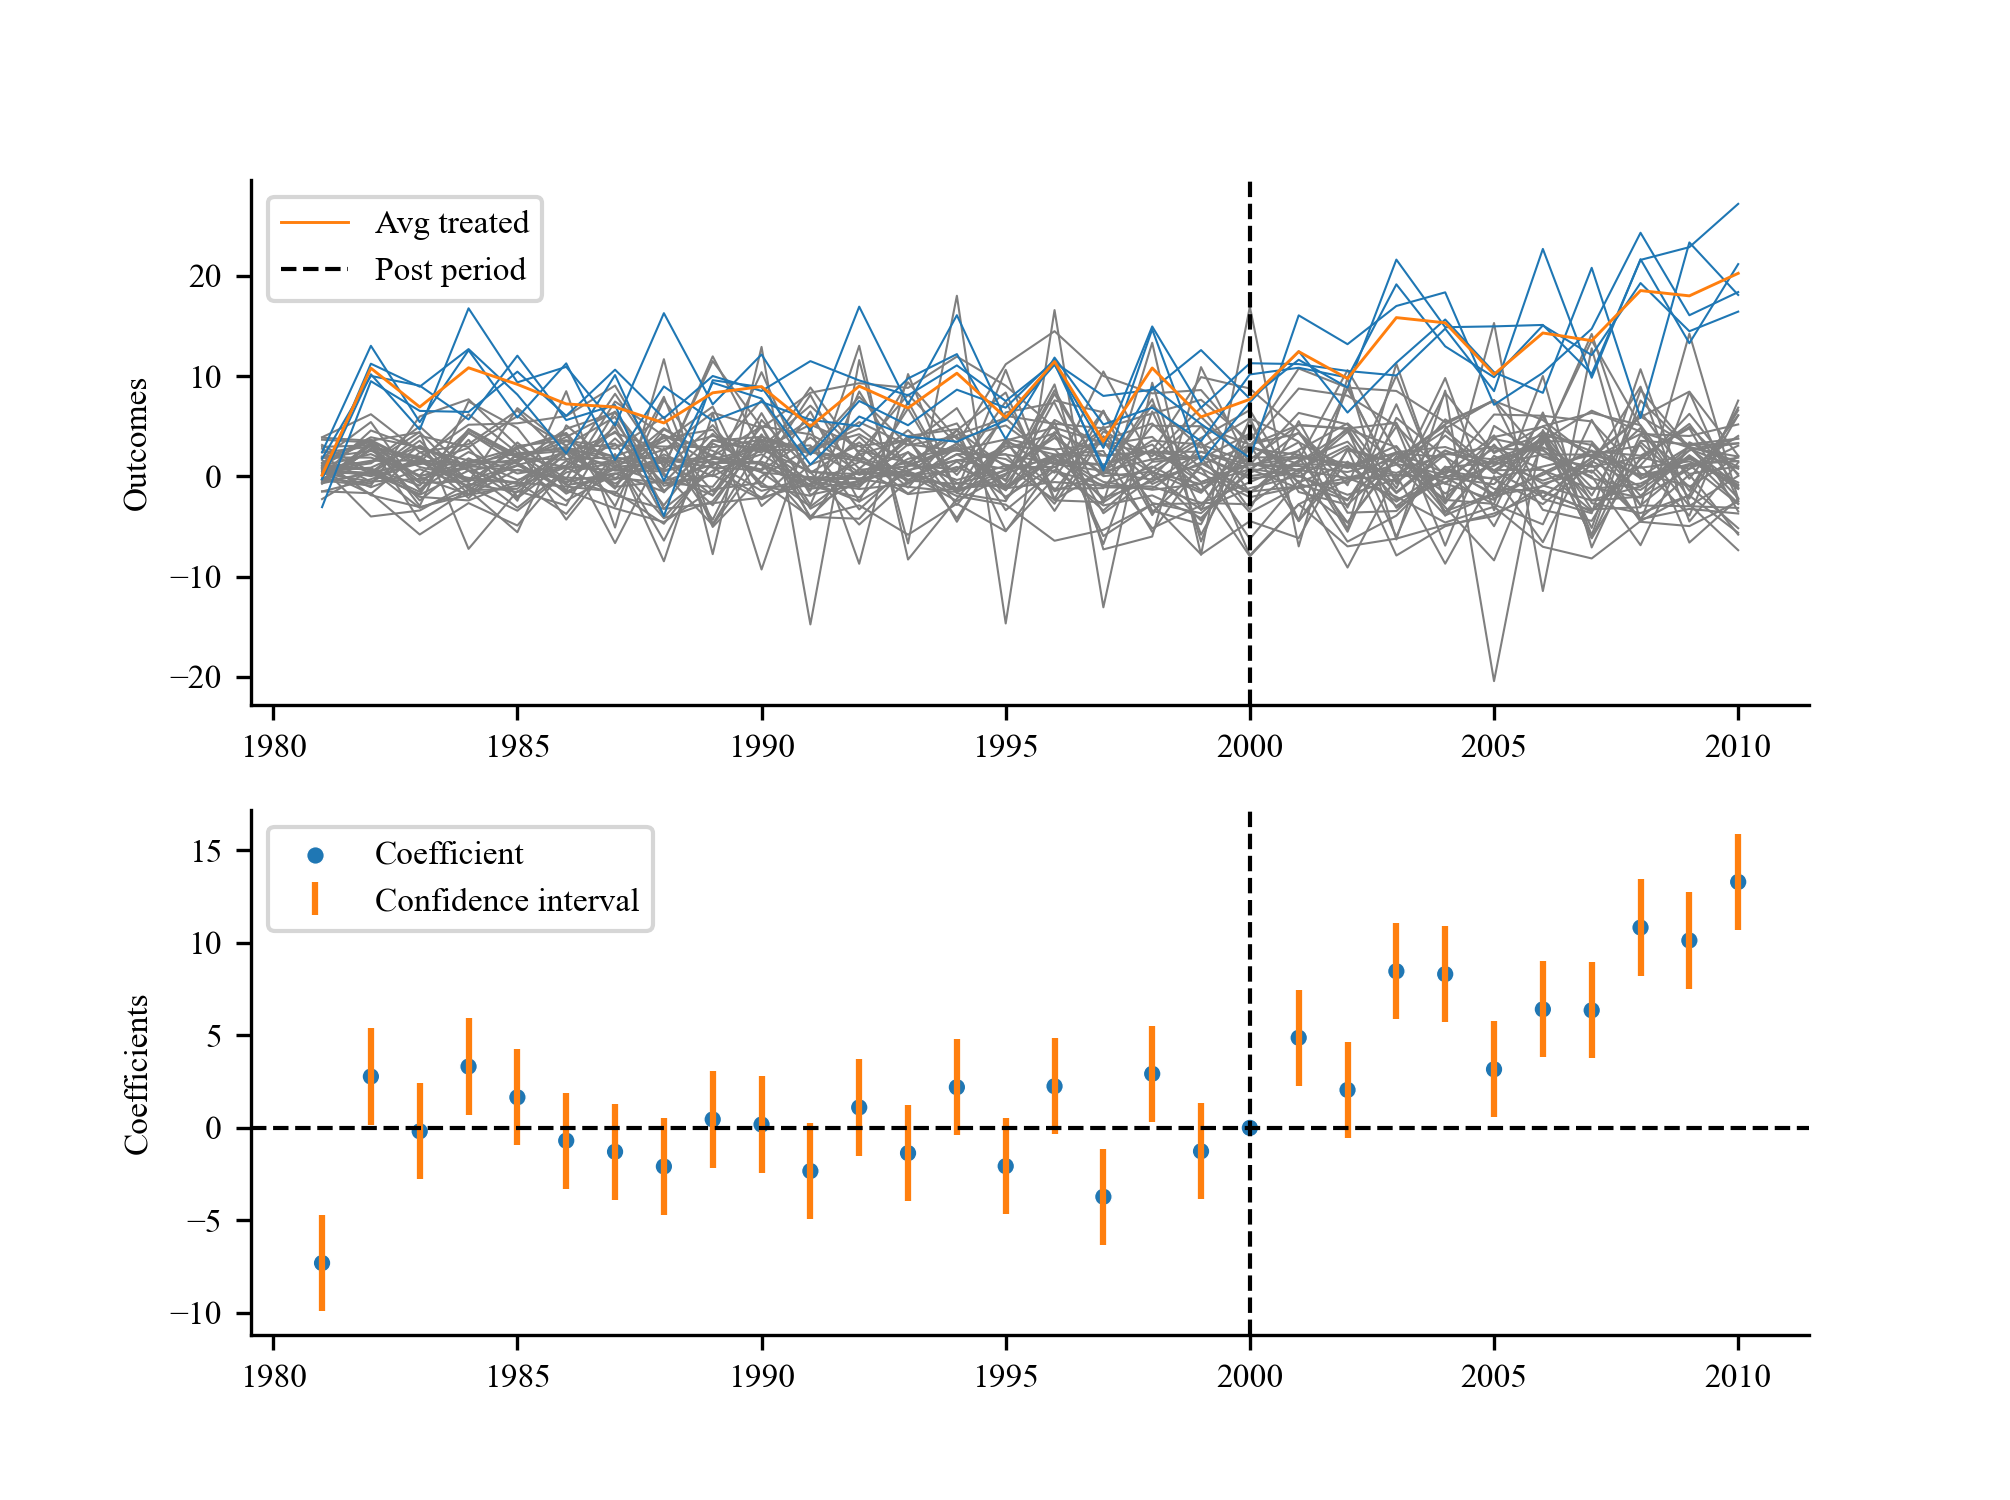
\includegraphics{figs/data_plot.png}
    \label{fig: sim}
    \caption*{\footnotesize{In this graphic, the upper panel plots simulated data following the above data generating process. The light blue lines represent treated units and the light gray lines represent controls. Key parameters are $N_{treat} = 5, N_{ctrl} = 45, T_0=20, T_1=10, L=10$. The lower panel plots a simple event study.}}
    \end{figure}

Figure \ref{fig: sim} represents the simulated data following our data generating process. Observations from the upper panel indicate that the parallel trend assumption is not met. To verify this, we plot a simple event study, clearly revealing a failure in the parallel trend assumption. Furthermore, outcomes for treated units are marginally higher than for control units. In such cases, the synthetic control method will be biased, as it avoids extrapolation and typically fit poorly for treated units.

\subsection{A simulated example}
Following this data generating process, figure \ref{fig: est} illustrates both the raw data and the imputed counterfactual outcomes as estimated by the CSC-IPCA method. In the upper panel, control units are represented in gray and treated units in light blue, with the average outcome for treated units highlighted in orange. The imputed synthetic average for treated outcomes is also shown, delineated by an orange dashed line. The CSC-IPCA method is capable of capturing the trajectory of the average outcome for treated units before treatement and we observe the divergence after the treatment. The lower panel of Figure \ref{fig: est} shows the estimated ATT (dashed line) with the true ATT (solid line) and the 95\% confidence interval based on confermal inference. The CSC-IPCA method is able to capture the true ATT, as evidenced by the close alignment between the dashed and solid lines. The confidence interval constructed through confermal inference is also accurate, as it encompasses the true ATT.

\begin{figure}[!ht]
    \centering
    \caption{\textbf{CSC-IPCA Estimated ATT for Simulated Sample}}
    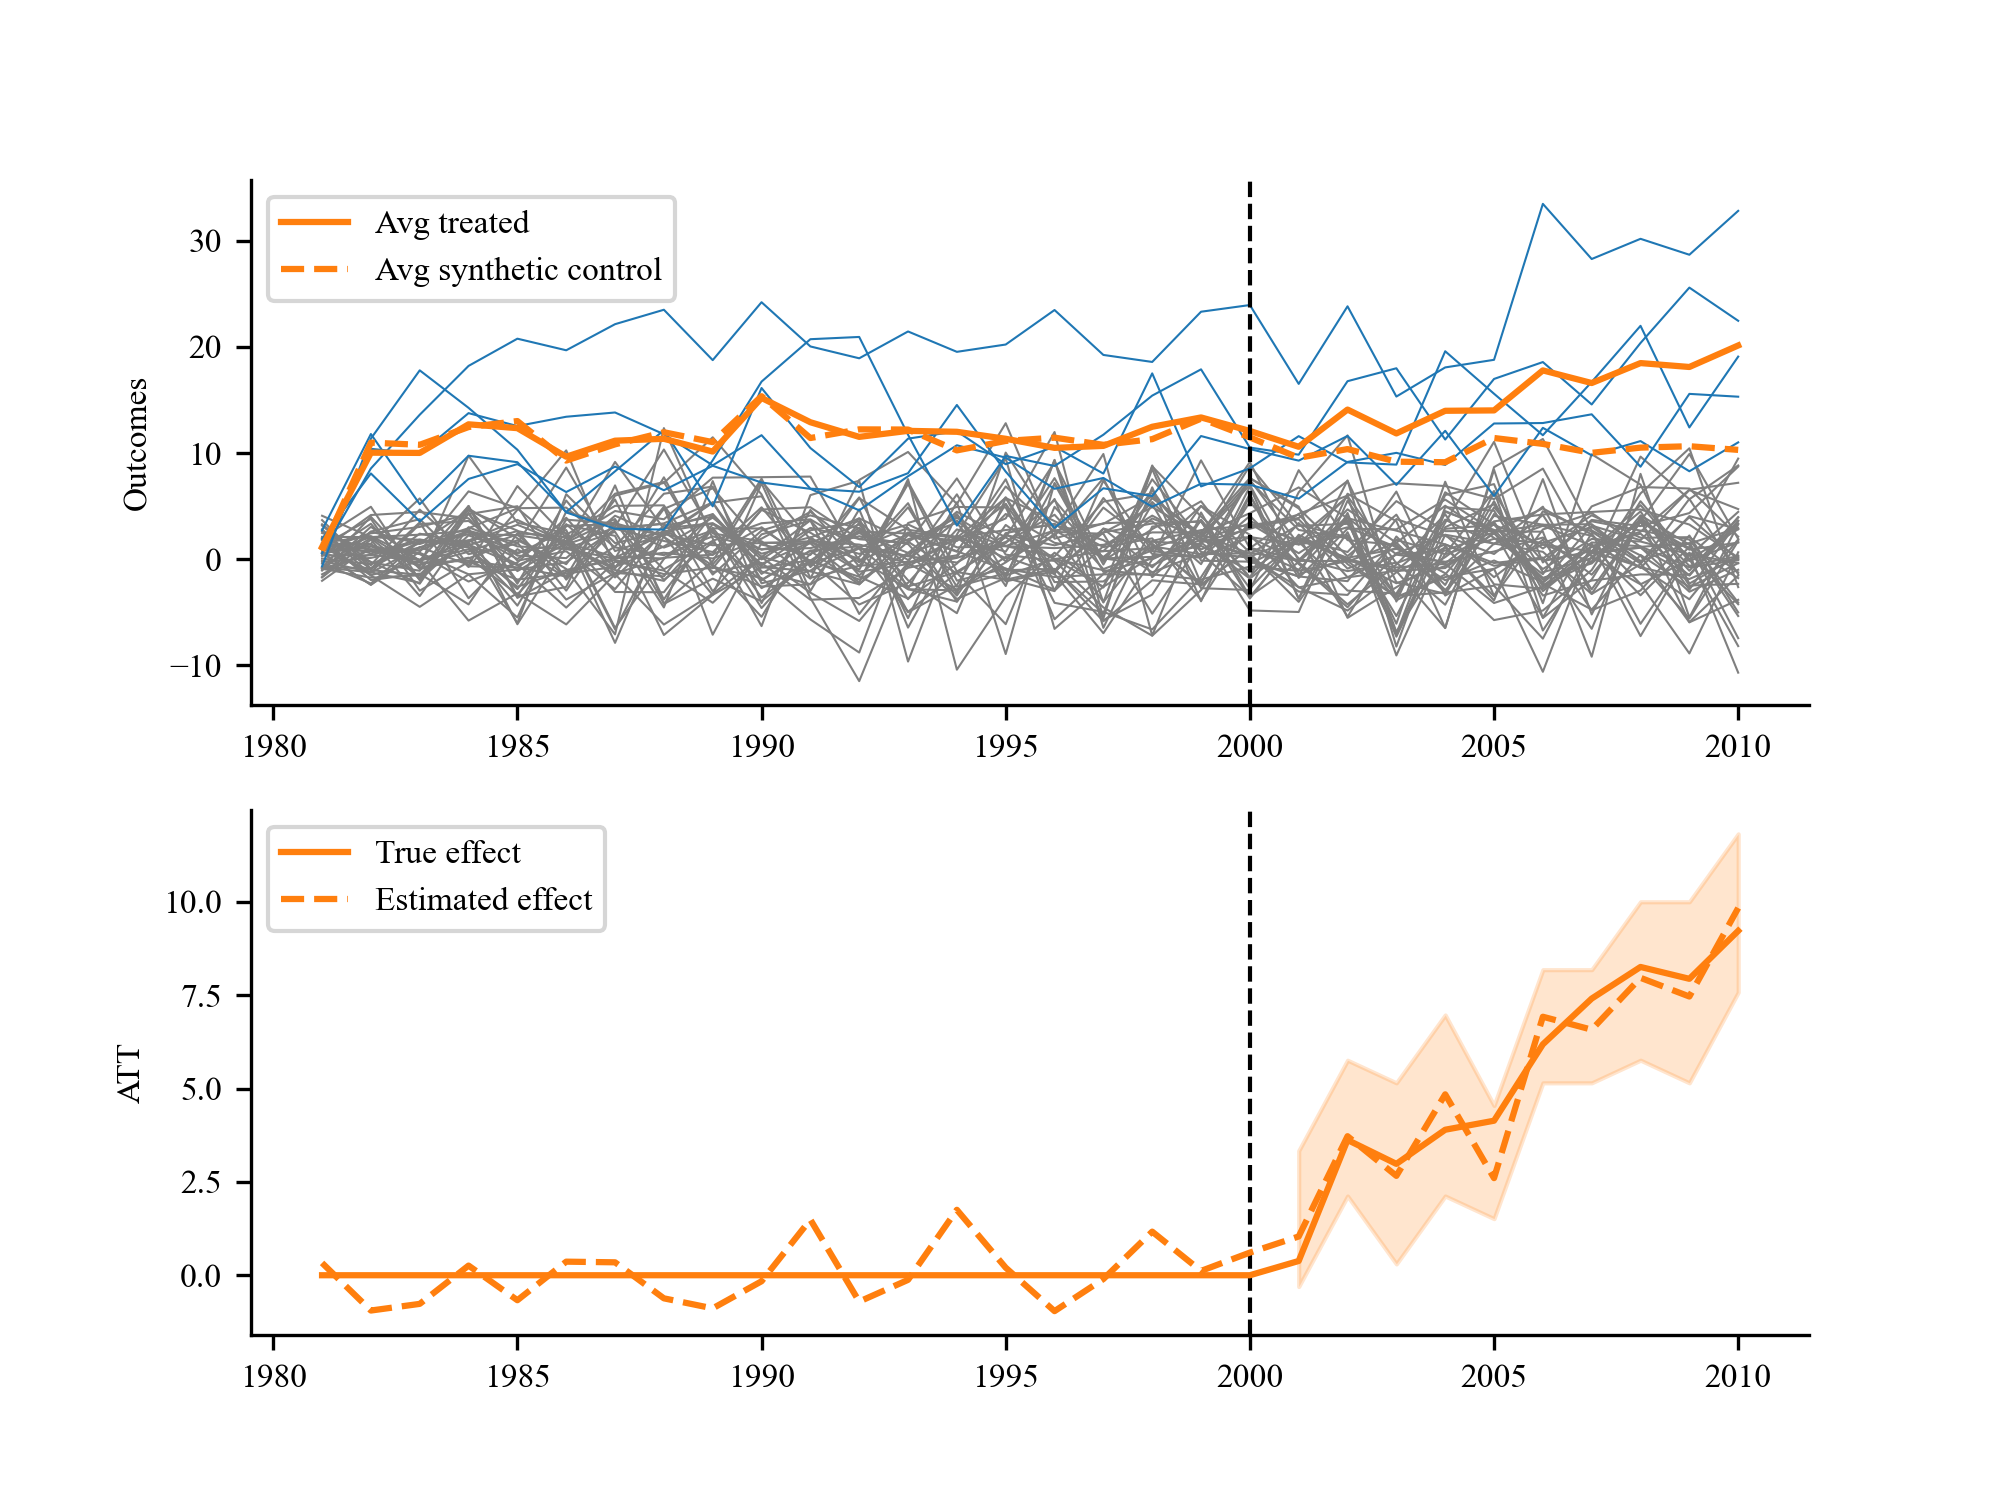
\includegraphics{figs/estimation.png}
    \label{fig: est}
    \caption*{\footnotesize{This graphic plots the CSC-IPCA method estimated ATT for simulated data $N_{treat} = 5, N_{ctrl} = 45, T_0=20, T_1=10, L=10$.}}
    \end{figure}

\subsection{Bias comparision}
Based on the same data generating process and parameters, we compare the CSC-IPCA, CSC-IFE, and SCM estimators with 1000 simulations. Figure \ref{fig: bias} illustrates the bias among these different estimation methods. In panel 1, when all covariates are observed, both CSC-IPCA and CSC-IFE demonstrate unbiasedness and effectively estimate the true ATT. However, due to the outcomes of treated units falling outside the convex hull of control units, the SCM exhibits an upward bias, as \cite{abadie2010synthetic} suggesting that in such senario we should avoiding SCM. It is often the case in financial and macroeconomic studies that we observe only a subset of covariates, rather than all of them. In panels 2 and 3, we observe only 2/3 and 1/3 of the covariates, respectively. As the number of unobserved covariates increases, both CSC-IPCA and CSC-IFE lose efficiency, but the CSC-IPCA estimator remains less unbiased than CSC-IPCA estimator. We compare the bias of different estimators with different DGPs in the Appendix \ref{app: bias 2}, and the results are consistent with the above findings.

\begin{figure}[!ht]
\centering
\caption{\textbf{Bias Comparing with Other Methods}}
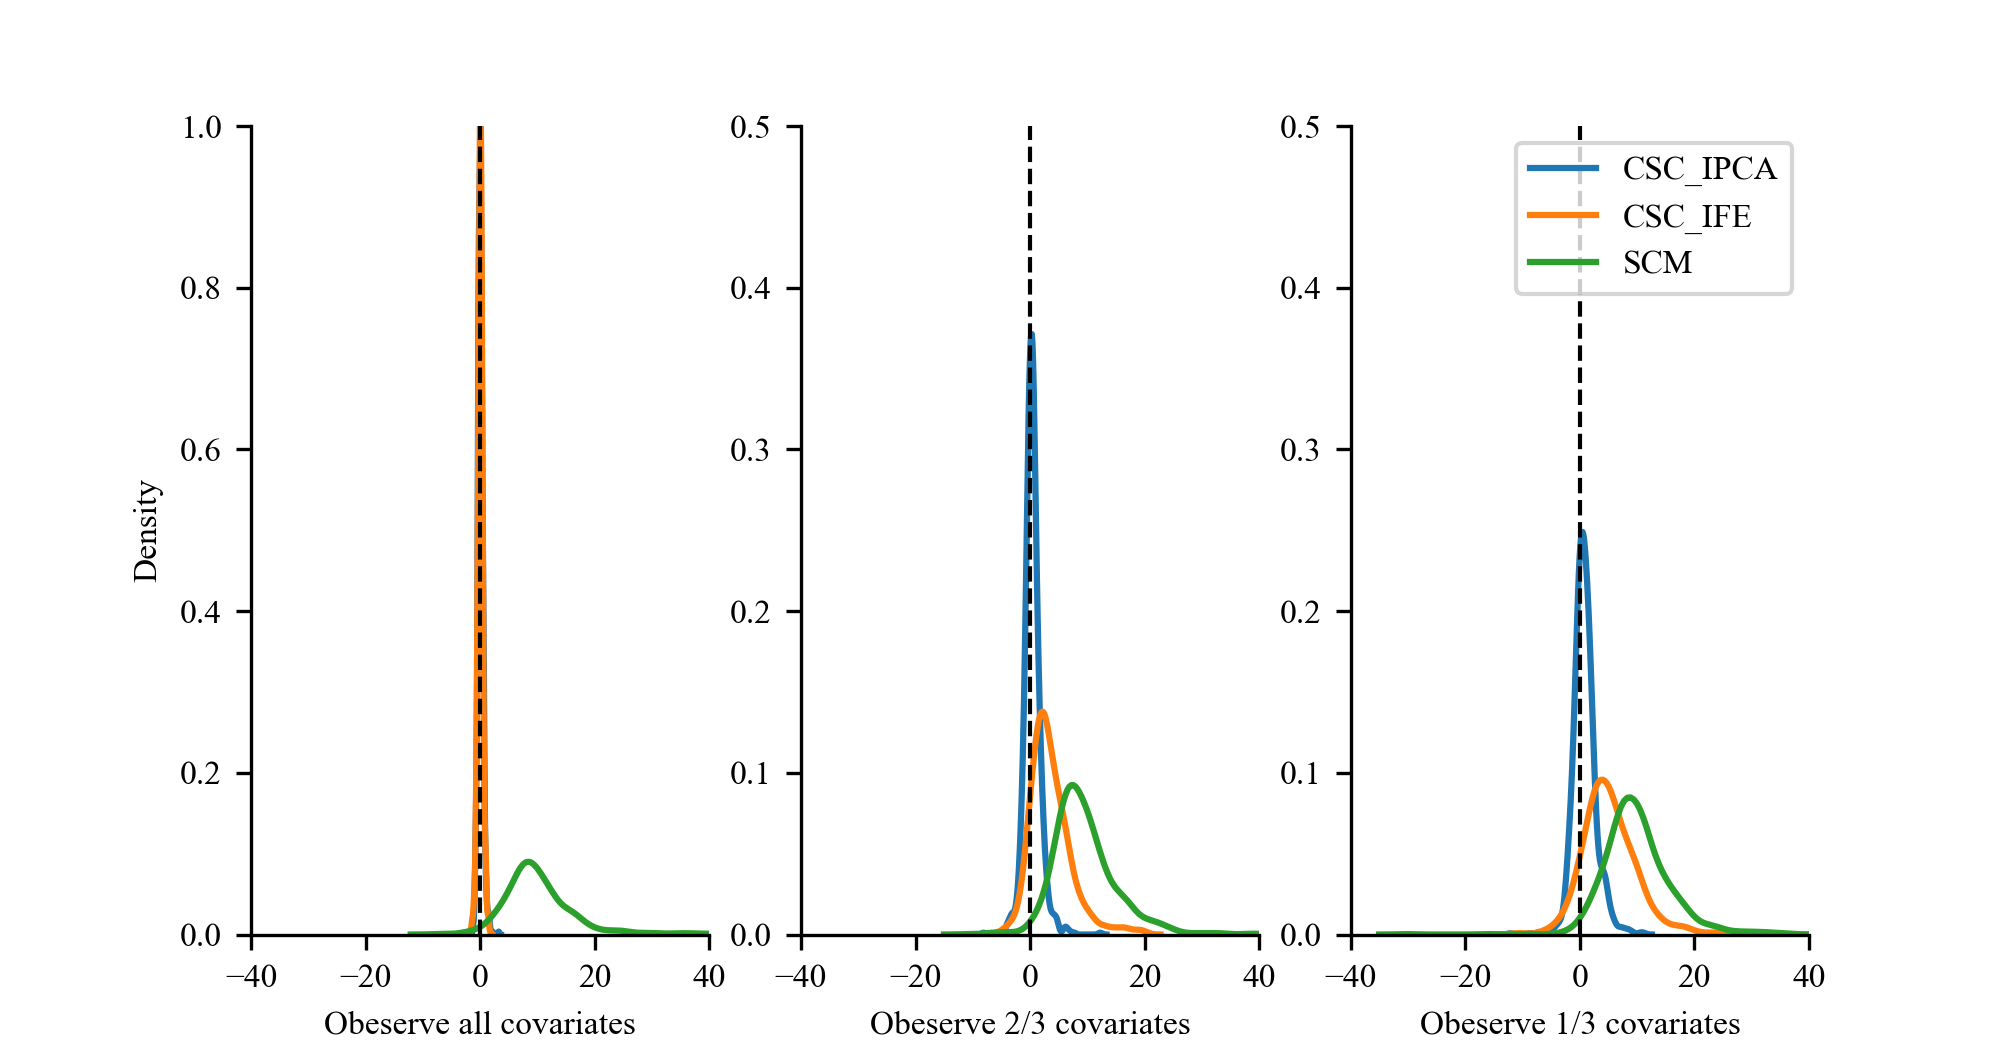
\includegraphics{figs/bias_compar1.png}
\label{fig: bias}
\caption*{\footnotesize{This graphic plots the bias of the CSC-IPCA, CSC-IFE, and SCM estimators for simulated data $N_{treat} = 5, N_{ctrl} = 45, T_0=20, T_1=10, L=10$.}}
\end{figure}

\subsection{Finite sample properties}
We present the Monte Carlo simulation results in Table \ref{tab: finite sample} to investigate the finite sample properties of the CSC-IPCA estimator. The numbers of treated units and post-treatment periods are fixed to $N_{treat} = 5, T_{post}=5$. We vary the number of control units $N_{ctrl}$, pre-treatment periods $T_{pre}$ , and the proportion of observed covariates $\alpha$ with the total number of covariates $L=9$ to investigate the finite sample properties. As showing in the table \ref{tab: finite sample}, the bias, RMSE, and STD are estimated based on 1000 simulations\footnote{The root mean squared error (RMSE) is defined as $RMSE = \sqrt{\frac{1}{T_{pre}}\sum_{t \in T_{pre}}\left(ATT_t - \widehat{ATT}_t\right)^2}$. The standard deviation (STD) is defined as $STD = \frac{1}{T_{pre}}\sum_{t \in T_{pre}}\left(\widehat{ATT}_t - \frac{1}{T_{pre}}\sum_{t \in T_{pre}}\widehat{ATT_t}\right)^2$}. The results indicate that the bias of the CSC-IPCA estimator decreases as the number of control units and pre-treatment periods increases. Suggested by the theoritical results, the convergence rate of the CSC-IPCA estimator is the smaller one between $\mathcal{O}_p\left(\sqrt{N_{ctrl}}\right)$ and $\mathcal{O}_p\left(\sqrt{N_{treat}T_{pre}}\right)$. In this simulation example, since the smaller one is always $\mathcal{O}_p\left(\sqrt{N_{ctrl}}\right)$ we observe that the bias decreases significantly when the number of control units increases from 10 to 40. The number of observed covariates also plays a crucial role in the bias reduction. The bias decreases the most when the proportion of observed covariates increases from $1/3$ to 1 (all covariates are observed). We observe similar pattern in RMSE and STD. It is worth noting that if we observe all the covariates (i.e., $\alpha = 1$), the bias, RMSE, and STD of the CSC-IPCA estimator are all reduce to the lowest level even with a small number of control units and pre-treatment periods. We present the finite sample properties of the CSC-IFE and SCM estimators in the Appendix \ref{app: finite sample}. When observe all the covariates, the CSC-IFE estimator is comparable to the CSC-IPCA estimator, however, when the number of observed covariates decreases, the CSC-IFE estimator is more biased than the CSC-IPCA estimator. The SCM estimator is always biased due to the settings.

\begin{table}[!ht]
    \centering
    \caption{\textbf{Finite Sample Properties}}
    \label{tab: finite sample}
    \begin{tabular}{cc|ccc|ccc|ccc}
    \toprule
    \multicolumn{2}{c|}{$\alpha$} & $1/3$ & $2/3$ & 1 & $1/3$ & $2/3$ & 1 & $1/3$ & $2/3$ & 1 \\
    \hline
    $T_0$ & $N_{ctrl}$ & \multicolumn{3}{c|}{Bias} & \multicolumn{3}{c|}{RMSE}  & \multicolumn{3}{c}{STD} \\
    \hline
    10 & 10 & 2.328 & 0.703 & 0.130 & 4.770 & 3.068 & 1.642 & 4.175 & 3.032 & 1.684 \\
    10 & 20 & 1.367 & 0.312 & 0.053 & 3.484 & 2.209 & 0.914 & 3.260 & 2.219 & 1.008 \\
    10 & 40 & 1.026 & 0.196 & 0.051 & 2.776 & 1.752 & 0.714 & 2.616 & 1.781 & 0.821 \\
    \cline{1-11}
    20 & 10 & 2.957 & 1.029 & 0.217 & 4.817 & 2.696 & 1.135 & 3.814 & 2.544 & 1.179 \\
    20 & 20 & 1.435 & 0.438 & 0.055 & 3.280 & 1.754 & 0.745 & 2.982 & 1.773 & 0.860 \\
    20 & 40 & 1.093 & 0.167 & 0.042 & 2.613 & 1.348 & 0.602 & 2.430 & 1.409 & 0.757 \\
    \cline{1-11}
    40 & 10 & 2.905 & 1.232 & 0.145 & 4.911 & 3.035 & 0.969 & 3.972 & 2.797 & 1.065 \\
    40 & 20 & 1.670 & 0.399 & 0.019 & 3.592 & 1.718 & 0.724 & 3.221 & 1.737 & 0.861 \\
    40 & 40 & 0.876 & 0.295 & 0.006 & 2.675 & 1.418 & 0.574 & 2.556 & 1.441 & 0.697 \\
    \bottomrule
    \end{tabular}
    \begin{tablenotes}
        \item This table presents the finite sample properties of the CSC-IPCA method estimated ATT for simulated data. The number of treated units and post-treatment period are fixed to $N_{treat} = 5, T_1=5$. We vary the number of control units $N_{ctrl}$, pre-treatment period $T_0$, and proportion of observed covariates $\alpha$ to investigate the finite sample properties, the total number of covariates is $L=9$. The bias, RMSE, and STD are estimated based on 1000 simulations.
    \end{tablenotes}
    \end{table}
%%%%%%%%%%%%%%%%%%%%%%%%%%%%%%%%%%%%%%%%%%%%%%%%%%%%%%%%%%%%%%%
%%%%%%%%%%%%%%%%%%%%%%%%%%%%%%%%%%%%%%%%%%%%%%%%%%%%%%%%%%%%%%%
\section{Empirical Application}
\label{sec: application}
%%%%%%%%%%%%%%%%%%%%%%%%%%%%%%%%%%%%%%%%%%%%%%%%%%%


%%%%%%%%%%%%%%%%%%%%%%%%%%%%%%%%%%%%%%%%%%%%%%%%%%%%%%%%%%%%%%%
%%%%%%%%%%%%%%%%%%%%%%%%%%%%%%%%%%%%%%%%%%%%%%%%%%%%%%%%%%%%%%%
\section{Conclusion} 
\label{sec: conclusion}
%%%%%%%%%%%%%%%%%%%%%%%%%%%%%%%%%%%%%%%%%%%%%%%%%%%%%%%


\clearpage
%%%%%%%%%%%%%%%%%%%%%%%%%%%%%%%%%%%%%%%%%%%%%%%%%%%%%%%%%%%%%%%
%%%%%%%%%%%%%%%%%%%%%%%%%%%%%%%%%%%%%%%%%%%%%%%%%%%%%%%%%%%%%%%
\begingroup
\setstretch{1.0}
\bibliographystyle{plainnat}
\bibliography{citation}
\endgroup

\clearpage
%%%%%%%%%%%%%%%%%%%%%%%%%%%%%%%%%%%%%%%%%%%%%%%%%%%%%%%%%%%%%%%
%%%%%%%%%%%%%%%%%%%%%%%  Appendix  %%%%%%%%%%%%%%%%%%%%%%%%%%%%
%%%%%%%%%%%%%%%%%%%%%%%%%%%%%%%%%%%%%%%%%%%%%%%%%%%%%%%%%%%%%%%
\appendix
\titleformat{\section}[block]{\normalfont\Large\bfseries}{Appendix \thesection}{1em}{}
\renewcommand{\theequation}{\thesection.\arabic{equation}}
\setcounter{equation}{0}
\renewcommand{\theassumption}{\thesection.\arabic{assumption}}
\setcounter{assumption}{1}
\renewcommand{\thefigure}{\thesection.\arabic{figure}}
\setcounter{figure}{0}
%%%%%%%%%%%%%%%%%%%%%%%%%%%%%%%%%%%%%%%%%%%%%%%%%%%%%%%%%%%%%%%

\section{Technical Details}
\label{sec: appendix}

\subsection{Treatment Assignment}
\label{app: treatment assignment}
%%%%%%%%%%%%%%%%%%%%%%%%%%%%%%%%%%%%%%%%%%%%%%%%%%%

To simplify the computation, we assume that the treatment assignment is based on a block assignment mechanism. 

\begin{figure}[!ht]
\centering
\caption{\textbf{Block Assignment}}
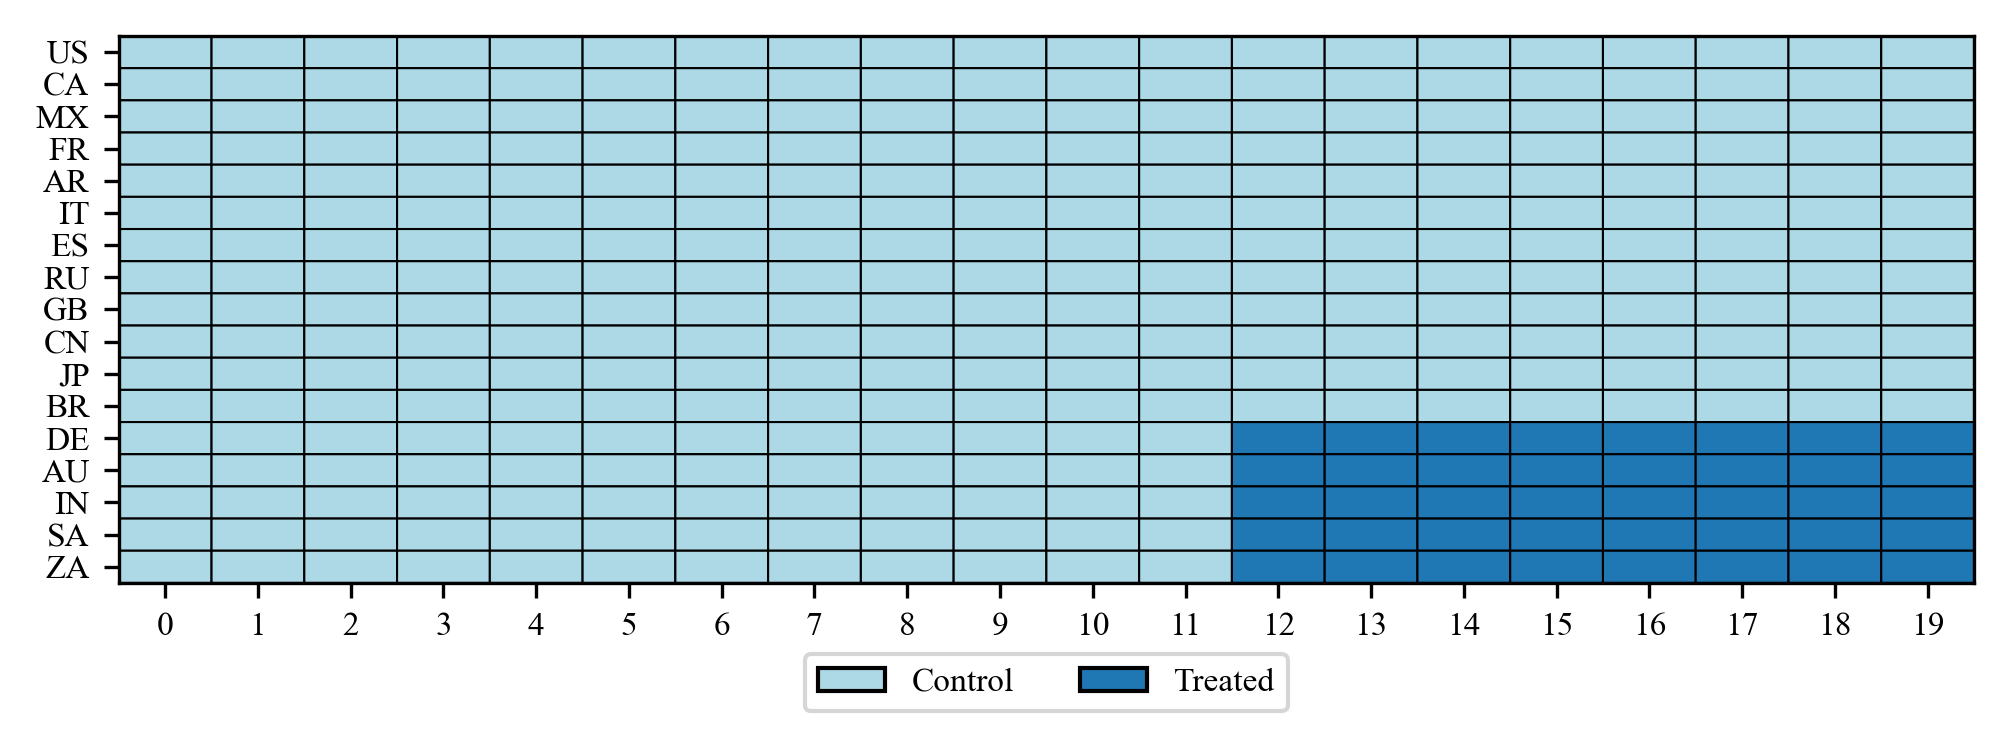
\includegraphics{figs/block_assignment.png}
\label{app: block assignment}
\caption*{\footnotesize{This graphic depicts the block assignment mechanism. Control units remain untreated throughout, while treated units receive the intervention simultaneously. Once the treatment is initiated, it is maintained permanently and cannot be reversed.}}
\end{figure}

The CSC-IPCA method can also be applied to estimate the staggered adoption mechanism, where treated units receive the intervention at different time points. The most complex scenario is the random assignment, where the treatment assignment is random and can be switched on or off at any time. This topic is beyond the scope of this paper, but matrix completion with nuclear norm, as detailed in \cite{athey2021matrix}, is a suitable approach for such cases.

\begin{figure}[!ht]
\centering
\caption{\textbf{Staggered Adoption}}
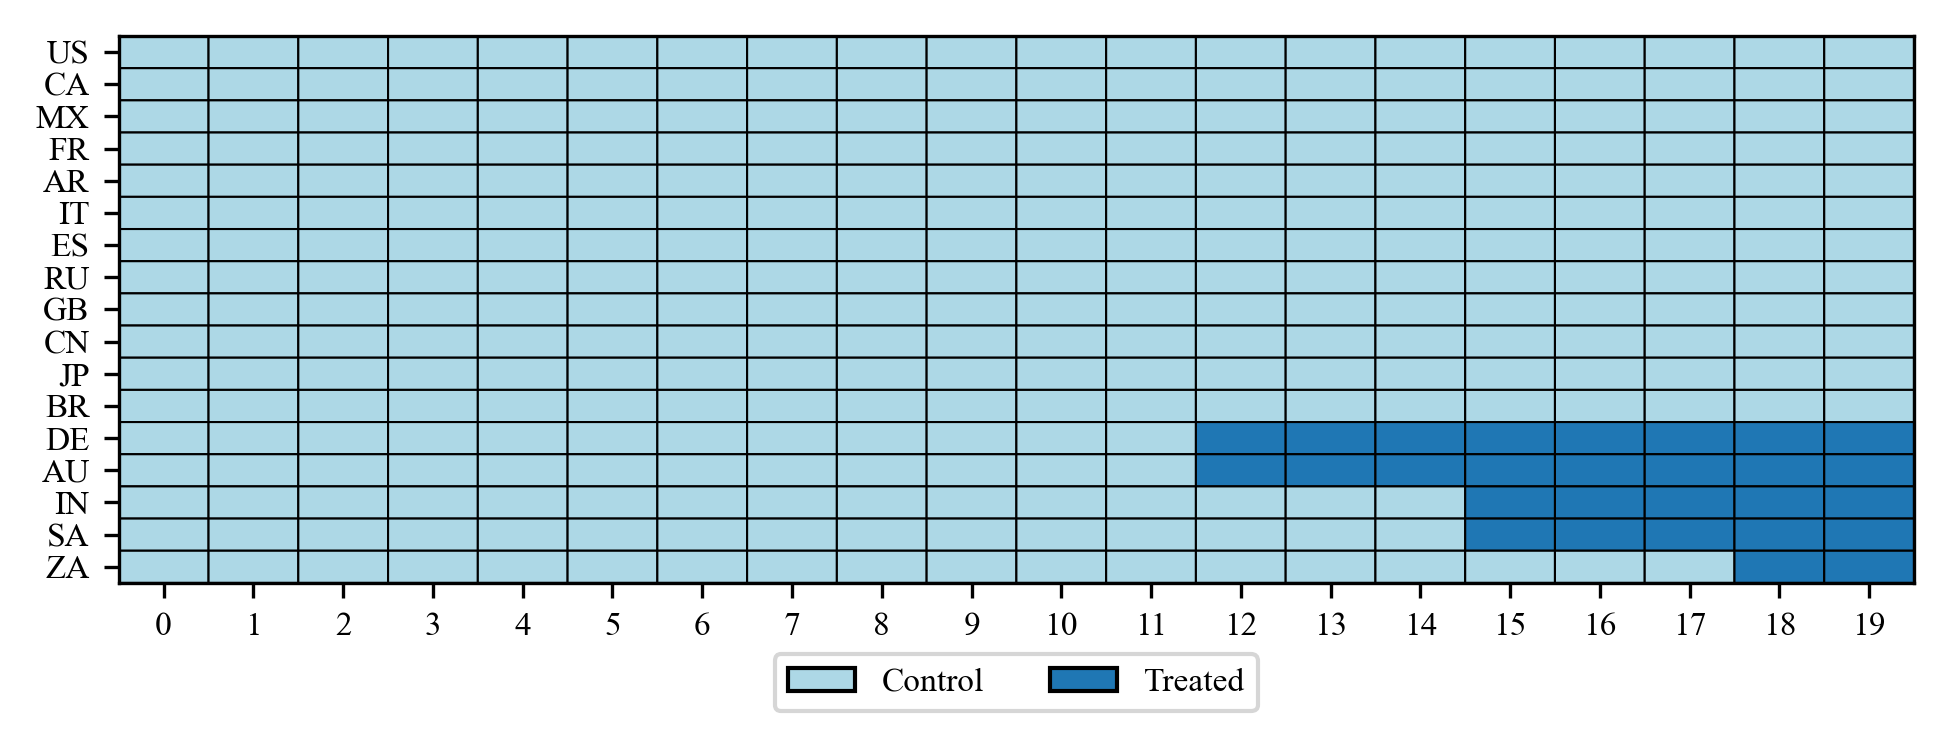
\includegraphics{figs/staggered_adoption.png}
\label{app: staggered adoption}
\caption*{\footnotesize{This graphic presents the staggered adoption mechanism. Control units remain untreated throughout, while treated units receive the intervention at different time points. Once the treatment is initiated, it is maintained permanently and cannot be reversed.}}
\end{figure}

\begin{figure}[!ht]
\centering
\caption{\textbf{Random Assignment}}
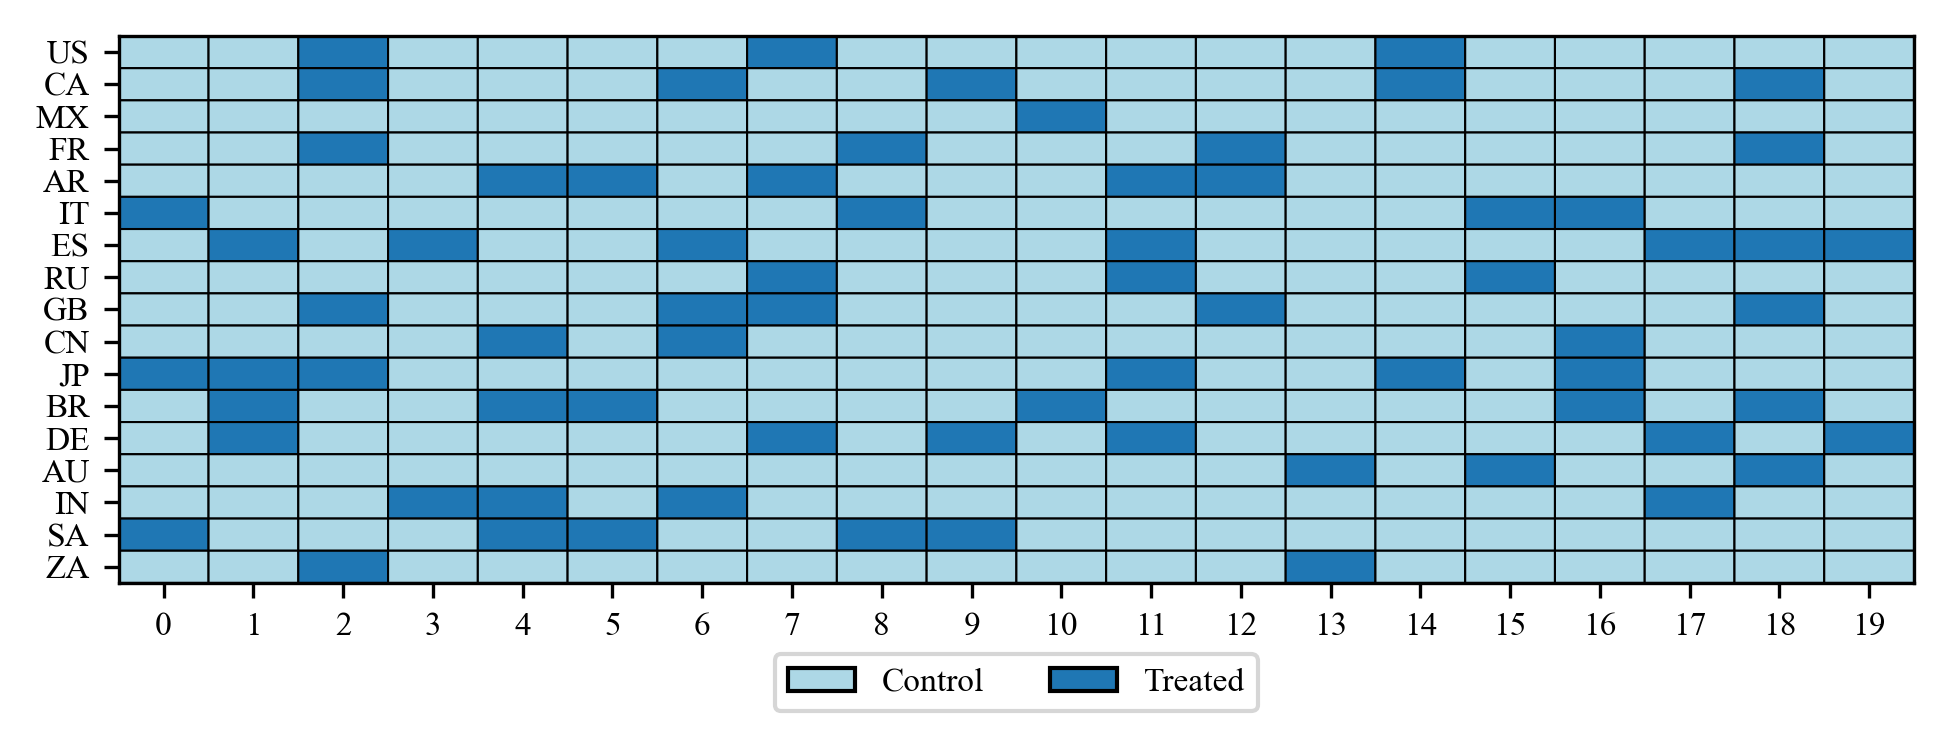
\includegraphics{figs/random_assignment.png}
\label{app: random assignment}
\caption*{\footnotesize{This graphic illustrates the random assignment mechanism. All units are randomly assigned to either the control or treatment group. The treatment can be switched on or off at any time.}}
\end{figure}

\subsection{Identification assumptions}

Following this section, we use lowercase letters to represent scalars, e.g., $y_{it}$ would be a scalar of the outcome variable for unit $i$ at time $t$. We use bold lowercase letters to represent vectors, e.g., $\bm{x}_{it}$ would be a vector of covariates for unit $i$ at time $t$. We use uppercase letters to represent matrices, e.g., $\Gamma$ represents the mapping matrix. We denote $\mathbb{E}\|\bm{f}_t\bm{f}_t'\|^2$ the Frobenius norm squared of the matrix $\bm{f}_t\bm{f}'_t$.

\begin{assumption}
Assumption for consistency:
\begin{enumerate}
    \item Covariate orthogonality: $\mathbb{E}\left[\textbf{x}'_{it} \epsilon_{it}\right] = \textbf{0}_{L\times 1}$,
    
    \item The following moments exist: $\mathbb{E}\|\bm{f}_{t}\bm{f}'_{t}\|^2$, $\mathbb{E}\|\bm{x}'_{it}\epsilon_{it}\|^2$, $\mathbb{E}\|\bm{x}'_{it}\bm{x}_{it}\|^2$, $\mathbb{E}\left[\|\bm{x}'_{it}\bm{x}_{it}\|^2\|\bm{f}_{t}\bm{f}'_{t}\|^2 \right]$, 

    \item Almost surely, $\bm{x}_{it}$ is bounded, and define $\Omega_t^{xx} := \mathbb{E}\left[ \bm{x}_{it}' \bm{x}_{it} \right]$, then almost surely, $\Omega_t^{xx} > \epsilon$ for some $\epsilon > 0$.
    
    \item The parameter space $\Psi$ of $\Gamma$ is compact and away from rank deficient: $\det{\Gamma' \Gamma} > \epsilon$ for some $\epsilon>0$,
    
\end{enumerate}
\label{app: ass consistency}
\end{assumption}

\begin{assumption}
Assumptions for asymptotic normality:
\begin{enumerate}
    \item $\text{As } N, T \to \infty, \: \frac{1}{\sqrt{NT}} \sum_{i,t} \text{vect}\left( \bm{x}'_{i,t} \epsilon_{i,t} \bm{f}'_{t} \right) \xrightarrow{d} \text{Normal} \left(0, \Omega^{x\epsilon f} \right)$,
    
    \item $\text{As } N \to \infty, \: \frac{1}{\sqrt{N}} \sum_{i} \text{vect}\left( X'_{i} \epsilon_{i} \right) \xrightarrow{d} \text{Normal} \left(0, \Omega^{x\epsilon} \right) \: \text{for} \: \forall t$,
    
    \item $\text{As } N, T \to \infty, \: \frac{1}{\sqrt{T}} \sum_{t} \text{vect}\left( \bm{f}_{t}\bm{f}'_{t} - \mathbb{E}[\bm{f}_{t}\bm{f}'_{t}] \right) \xrightarrow{d} \text{Normal} \left(0, \Omega^{f} \right)$.
    
    \item Bounded dependence: $\frac{1}{NT} \sum_{i,j,t,s}\|\tau_{ij, ts}\| < \infty$, where $\tau_{ij, ts} := \mathbb{E} \left[ \bm{x}'_{it} \epsilon_{it} \epsilon'_{js} \bm{x}_{js} \right]$
    
    \item Constant second moments of the covariates: $\Omega_t^{xx} = \mathbb{E}\left[ X_{t} X'_{t} \right]$ is constant across time periods.
    \end{enumerate}
    \label{app: ass normality}
\end{assumption}

\subsection{Estimation of the CSC-IPCA estimator}
\label{sec: appendix estimation}

As outlined in Equation \ref{eqn: functional form}, the structural components of the data generating process are constructed by the interactive fixed effect between time-varying factors $\bm{f}_t$ and dynamic factor loadings $\bm{\lambda}_{it}$, which is instrumented by the covariates $\bm{x}_{it}$ through the mapping matrix $\Gamma$. The data generating process can be formulated as follows:

\begin{equation}
\label{app: eqn combined}
y_{it} = (\bm{x}_{it}\Gamma) \bm{f}'_{t} + \epsilon_{it}, \quad \epsilon_{it} = \mu_{it} + \bm{h}_{it} \bm{f}'_t.
\end{equation}

where the error term $\epsilon_{it}$ is combined with the interaction between time-varying factors $\bm{f}_t$ and error term associated with factor loadings $\bm{h}_{it}$ and the idiosyncratic error $\mu_{it}$. The objective function in Equation \ref{eqn: obj} is minimized to estimate the factor $\bm{f}_t$ and mapping matrix $\Gamma$. Equation \ref{app: eqn first step} details the first step to estimate the factor $\bm{f}_t$ and mapping matrix $\Gamma$ with only the control units:

\begin{equation}
\label{app: eqn first step}
(\hat{\Gamma}_{ctrl}, \hat{\bm{f}}_t) = \underset{\Gamma, \bm{f}_t}{\arg\min} \sum_{i \in \mathcal{T}} \sum_{t \leq T} \left( y_{it} - (\bm{x}_{it}\Gamma) \bm{f}'_{t} \right)' \left( y_{it} - (\bm{x}_{it}\Gamma) \bm{f}'_{t} \right).
\end{equation}

The alternating least squares (ALS) method is employed for the numerical solution of this optimization problem. Unlike PCA, the IPCA optimization challenge cannot be resolved through eigen decomposition. The optimization, as defined in the equation above, is quadratic with respect to either $\Gamma$ or $\bm{f}_t$, when the other is held constant. This characteristic permits the analytical optimization of $\Gamma$ and $\bm{f}_t$ sequentially. With a fixed $\Gamma$, the solutions for $\bm{f}_t$ are t-separable and can be obtained via cross-sectional OLS for each $t$:

\begin{equation}
\label{app: eqn update f}
\hat{\bm{f}}_t(\Gamma) = (\Gamma' \bm{x}'_t \bm{x}_t \Gamma)^{-1} \Gamma' \bm{x}'_t y_t.
\end{equation}

Conversely, with known $\bm{f}_{t}$, the optimal $\Gamma$ (vectorized as $\bm{\gamma} = vect(\Gamma)$) is derived through pooled OLS of $y_{it}$ against $LK$ regressors, $\bm{x}_{it} \otimes \bm{f}_t$:

\begin{equation}
\label{app: eqn update gamma}
\hat{\gamma} = \left( \sum_{i,t} (\bm{x}_{i,t}' \otimes \bm{f}_t) (\bm{x}_{i,t} \otimes \bm{f}_t') \right)^{-1} \left( \sum_{i,t} (\bm{x}_{i,t}' \otimes \bm{f}_t) y_{i,t} \right).
\end{equation}

Inspired by PCA, the initial guess for $\bm{f}_t$ is the first $K$ principal components of the $N \times T$ outcome matrix $Y$\footnote{Here we remove the subscripte ``$it$'' indicating that matrix $Y$ represents the panel outcome of all units across all time periods.}. The ALS algorithm alternates between these two steps until convergence is achieved, typically reaching a local minimum rapidly. The convergence criterion, based on the minimization of relative change in the parameters $\bm{f}_t$ and $\Gamma$ in each iteration, ensures termination when this change falls below a predefined threshold, set at $1e-6$ in our implementation.

As we have mentioned before the estimation of $\bm{f}_{t}$ and $\Gamma$ is not deterministic. \cite{bai2009panel} and \cite{xu2017generalized} set the constraints on the factor loadings and factors before the estimation to ensure the identifiability of the model. However, in our case, since the structural component is identified by the product between factors and factor loadings $\bm{x}_{it}\Gamma \bm{f}'_{t}$, we can find any arbitrary rotation matrix $R$, such that $\bm{x}_{it}\Gamma R R^{-1}\bm{f}'_{t}$ yields the same structural component. For a specific constraints on the mapping matrix $\Gamma_{norm} = \Gamma_{treat}R$ and factor $\bm{f}_{norm} = R^{-1}\bm{f}_t$, such that:

\begin{equation}
\begin{aligned}
& \Gamma_{norm}'\Gamma_{norm} = \mathcal{I}_K, \\
& \bm{f}_{norm} \bm{f}_{norm}'/T = \text{Diagonal}.
\end{aligned}
\end{equation}

where $\mathcal{I}_K$ is a $K \times K$ identity matrix, and $T$ is the number of time periods. The rotation matrix $R$ can be easily found by the following steps: first, we use Cholesky decomposition (referred to \cite{higham2009cholesky} for a guidence) to decompose the product $\Gamma' \Gamma$ into a upper triangular matrix $R_1 = cholesky(\Gamma' \Gamma)$, then we perform singular value decomposition on $R_1\bm{f}_t\bm{f}_t'R_1'$ to get $R_2 = U$ where $U\Sigma V'=svd(R_1\bm{f}_t\bm{f}_t'R_1')$. Finally, the rotation matrix $R$ is given by:

\begin{equation}
R = R_1^{-1}R_2.
\end{equation}

\subsection{Hyperparameter tuning}
\label{sec: appendix hyperparameter}
We can also utilize leave-one-out cross validation to select the hyperparameter $K$, as detailed in Algorithm \ref{algorithm: 2}. This method involves excluding the $t^{th}$ period data from the control group to serve as the training data, while similarly excluding the corresponding period data from the treated group to act as validation data. This process is repeated for each time period in the pretreatment phase, applying a predetermined number of factor loadings. The optimal number of factors, $K$, is identified as the one that yields the minimum average of sum squared errors across all iterations.

\begin{algorithm}[!ht]
    \SetAlgoLined
    \KwData{$Y, X$}
    \KwResult{Optimal hyperparameter $k$}
    Determine the maximum possible hyperparameter $K$\;
    Initialize an array $MSE$ to store the average of sum squared error for each $k$\;
     \For{$k=1$ to $K$}{
        Set sum of squared errors $SSE_k = 0$\;
        \For{$t \leftarrow 1$ to $T_{pre}$}{
            Remove the $t^{th}$ period observation from control data, using the rest as training data $(Y_{ctrl}^{-t}, X_{ctrl}^{-t})$\;
            
            Similarly, exclude the $t^{th}$ period observation from treated data, using the rest as validation data $(Y_{treat}^{-t}, X_{treat}^{-t})$\;
            
            Estimate parameters $\Gamma$ and $F_t$ using the training data via the ALS method\;
            
            Use the estimated $\hat{\Gamma}$ and $\hat{F}_t$ to predict $\hat{Y}^{-t}_{treat}$ with the validation data\;
            
            Calculate the sum squared error $SE_t = \sum (Y_{treat}^{-t} - \hat{Y}_{treat}^{-t})^2$\;
            
            Accumulate the sum of squared errors:  $SSE_k \leftarrow SSE_k + SE_t$\;
        }
        Calculate the average sum squared error for $k$: $MSE[k] = \frac{SSE_k}{T_{pre}}$\;
      }
      Select $k$ corresponding to the minimum value in $MSE$\;
    \caption{Leave-One-Out Cross-Validation for Hyperparameter $k$}
    \label{algorithm: 2}
\end{algorithm}

%%%%%%%%%%%%%%%%%%%%%%%%%%%%%%%%%%%%%%%%%%%%%%%%%%%%%%%%%%%%%%%
\section{Formal Result}
\label{sec: formal result}
%%%%%%%%%%%%%%%%%%%%%%%%%%%%%%%%%%%%%%%%%%%%%%%%%%%
In this section, we derive the formal result for the CSC-IPCA estimator. We first establish the consistency and asymptotic properties of the mapping matrix $\Gamma$ and the factor $\bm{f}_t$. We then derive the formal result for the CSC-IPCA estimated ATT. 

\subsection{Mapping matrix estimation asympototic properties}
%%%%%%%%%%%%%%%%%%%%%%%%%%%%%%%%%%%%%%%%%%%%%%%%%%%
In this section, we delve into the asymptotic properties of the estimation error associated with the mapping matrix. \cite{kelly2020instrumented} have proven it in their paper, referring to Theorem 3. The following proposition \ref{prop: gamma}, is a special case of their result. Based on our estimation methods, we estimate the mapping matrix $\Gamma$ first by concentrating out the factor $\bm{f}_t$, as shown in Equation \ref{eqn: obj}, we can formulate a target function for $\Gamma$ as follows:

\begin{equation}
\label{eqn: target}
G(\Gamma) = \frac{1}{2NT}\sum_{i,t} \left( y_{it} - \bm{x}_{it}\Gamma \bm{\hat{f}}_t \right)^2.
\end{equation}
we define the score function $S(\Gamma)$ as the derivative of the target function $G(\Gamma)$ with respect to $\Gamma$: $S(\Gamma) = \frac{\partial G(\Gamma)}{\partial \Gamma}$. The Hessian matrix $H(\Gamma)$ is defined as the second derivative of the target function $G(\Gamma)$ with respect to $\Gamma$: $H(\Gamma) = \frac{\partial^2 G(\Gamma)}{\partial \Gamma \partial \Gamma'}$. 

It is crucial to highlight that our normalization criterion, delineated in Equation \ref{eqn: normalization}, mandates that the mapping matrix $\Gamma$ adheres to orthonormality and the factor $\bm{f}_t\bm{f}_t'/T$ is required to exhibit orthogonality. To satisfy these requirement we define the following identification function:
\begin{equation}
\label{eqn: identification}
I(\Gamma) := \begin{bmatrix}
    \text{veca}(\Gamma' \Gamma - \mathcal{I}_K) \\
    \text{vecb}\left(\frac{1}{T} \sum_{t} \bm{\hat{f}}_t\bm{\hat{f}}_t' - V^{ff}\right)
    \end{bmatrix}
\end{equation}
where $V^{ff} = E\left[\bm{f}_t\bm{f}'_t\right]$, meanwhile, $\text{veca}(\cdot)$ and $\text{vecb}(\cdot)$ vectorize the upper triangular entries of a square matrix. The difference is $\text{veca}(\cdot)$ includes the diagonal elements, while $\text{vecb}(\cdot)$ excludes them. We define the Jacobian matrix $J(\Gamma)$ as the derivative of the identification function $I(\Gamma)$ with respect to $\Gamma$: $J(\Gamma) = \frac{\partial I(\Gamma)}{\partial \Gamma}$.

\begin{proposition}
\label{prop: gamma}
Under Assumption \ref{app: ass consistency} and \ref{app: ass normality}, mapping matrix estimation error centered against the normalized true mapping matrix converges to a normal distribution at the rate of $\sqrt{NT}$: as $N, T \rightarrow \infty$ such that $T/N \rightarrow \infty$,

$$
\sqrt{NT} \left( \hat{\bm{\gamma}} - \bm{\gamma}^0 \right) \xrightarrow{d} - \left( H^{0'}H^0 + J^{0'}J^0 \right)^{-1}H^{0'}Normal(0, \mathbb{V}^{[1]})
$$
\end{proposition}
where $H^0:= \frac{\partial^2 G(\Gamma)}{\partial \bm{\gamma}\partial \bm{\gamma}'}|_{\bm{\gamma} = \bm{\gamma}^0}$ and $J^0:= \frac{\partial I(\Gamma)}{\partial \bm{\gamma}}|_{\bm{\gamma} = \bm{\gamma}^0}$, $\mathbb{V}^{[1]} = \left( Q^0 \otimes \mathcal{I}_K \right) \Omega^{x\epsilon f} \left( Q^{0'} \otimes \mathcal{I}_K \right)$, and $Q^0 := Q_t(\Gamma^0)$ given that $Q_t(\Gamma) := \mathcal{I}_L - \Omega_t^{xx} \left( \Gamma' \Omega^{xx}_t \Gamma \right)^{-1}\Gamma'$ is constant over $t$ under Assumption \ref{app: ass normality}.

\textbf{Proof}: referring to \cite{kelly2020instrumented}.
\subsection{Factor estimation asympototic properties}
%%%%%%%%%%%%%%%%%%%%%%%%%%%%%%%%%%%%%%%%%%%%%%%%%%%
\begin{proposition}
\label{prop: factor}
Under Assumption \ref{app: ass consistency} and \ref{app: ass normality}, factor estimation error centered against the normalized true factor converges to a normal distribution at the rate of $\sqrt{N}$: as $N, T \to \infty$ for $\forall t$,
$$
\sqrt{N}\left(\hat{\bm{f}}_t - \bm{f}^0_t\right) \xrightarrow{d} N\left(0, \mathbb{V}_t^{[2]}\right),
$$
\end{proposition}
where the variance term $\mathbb{V}_{t}^{[2]}$, which is given by $\mathbb{V}_{t}^{[2]} = \left( \Gamma^\top \Omega_{t}^{xx} \Gamma\right)^{-1} \Gamma^\top \Omega_{t}^{x\epsilon} \Gamma \left(\Gamma^\top\Omega_{t}^{xx} \Gamma\right)^{-1}$.

\textbf{Proof:} Decompose the left-hand side equation:
\begin{equation*}
\begin{aligned}
\sqrt{N}\left(\bm{\hat{f}}_t - \bm{f}_t\right) &= \sqrt{N}\left(\left( \hat{\Gamma}'X'_tX_t\hat{\Gamma} \right)^{-1}\hat{\Gamma}'X_t' \left(X_t\hat{\Gamma}\bm{f}_t+ \bm{\tilde{\epsilon}}_t \right) - \bm{f}_t\right)\\
&= \sqrt{N}\left(\left( \hat{\Gamma}'X'_tX_t\hat{\Gamma} \right)^{-1}\hat{\Gamma}'X_t' \left(X_t \hat{\Gamma}\bm{f}_t\right) - \bm{f}_t\right) + \sqrt{N}\left( \hat{\Gamma}'X'_tX_t\hat{\Gamma} \right)^{-1}\hat{\Gamma}'X_t'\bm{\tilde{\epsilon}}_t
\end{aligned}
\end{equation*}
where $\bm{\tilde{\epsilon}}_t$ is the estimated error term with estimated $\hat\Gamma$ and true $\bm{f}_t$. Given Proposition \ref{prop: gamma}, $\hat{\Gamma} - \hat{\Gamma}^0 = \mathcal{O}_p \left( 1/\sqrt{NT} \right)$. The first term is simply $\mathcal{O}_p\left(1/\sqrt{NT}\right)$. For the second term:

\begin{equation*}
\begin{aligned}
\sqrt{N}\left( \hat{\Gamma}'X'_tX_t\hat{\Gamma} \right)^{-1}\hat{\Gamma}'X_t'\bm{\tilde{\epsilon}}_t = &\sqrt{N}\left( \Gamma'X'_tX_t\Gamma \right)^{-1}\Gamma'X_t'\bm{\epsilon_t} + \mathcal{O}_p(1) \\
& \xrightarrow{d} Normal(0, \mathbb{V}_t^{[2]})
\end{aligned}
\end{equation*}

Assumption \ref{app: ass normality} delineates the properties of $\Omega_t^{xx}$ and $\Omega_t^{x\epsilon}$. Notably, despite the presence of multiple matrix multiplications, the matrices $\Omega_t^{xx}$ and $\Omega_t^{x\epsilon}$ remain invariant under these operations. Consequently, the term $\mathbb{V}_t^{[2]}$ is constant across all observational units.

%%%%%%%%%%%%%%%%%%%%%%%%%%%%%%%%%%%%%%%%%%%%%%%%%%%
\subsection{Consistency and asymptotic property of the ATT estimation}
%%%%%%%%%%%%%%%%%%%%%%%%%%%%%%%%%%%%%%%%%%%%%%%%%%%
\begin{theorem}
\label{thm: bias}
Under Assumptions \ref{ass: function}, \ref{app: ass consistency}, and \ref{app: ass normality}, the CSC-IPCA estimator $\mathbb{E}\left(\widehat{ATT}_{t} | D, X, \Gamma, F\right) \xrightarrow{P} ATT_{t}$, where $ATT_{t} = \frac{1}{N_{treat}}\sum_{i \in \mathcal{T}}\delta_{it}$ is the true treatment effect. for all $t > T_{pre}$ as both $N_{ctrl}, \ T_{pre} \to \infty$.
\end{theorem}

\textbf{Proof:} Denote $i$ as the treated unit on which the treatment effect is of interest, the bias of estimated ATT is given by:

\begin{equation*}
\begin{aligned}
\hat{\delta}_{it} - \delta_{it} &= y_{it}^1 - \hat{y}_{it}^0 - \delta_{it}, \\    
&= \textbf{x}_{it}\Gamma \bm{f}'_t - \textbf{x}_{it}\hat{\Gamma}\hat{\bm{f}}'_t + \epsilon_{it}, \\
&= \textbf{x}_{it}\left( \left(\mathcal{I}_L\otimes \bm{f}_t \right) \bm{\gamma} - (\mathcal{I}_L\otimes \hat{\bm{f}}_t ) \hat{\bm{\gamma}} \right) + \epsilon_{it}, \\
&= \textbf{x}_{it}\left( \left(\mathcal{I}_L\otimes \bm{f}_t \right) \bm{\gamma} - \mathcal{I}_L\otimes (\bm{f}_t + \bm{e}_{f_t}) (\bm{\gamma}+\textbf{e}_{\gamma}) \right) + \epsilon_{it}, \\
&= \textbf{x}_{it}\left( (\mathcal{I}_L \otimes \bm{f}_t) \textbf{e}_{\gamma} - (\mathcal{I}_L \otimes \bm{e}_{f_t} \bm{\gamma}) - (\mathcal{I}_L \otimes \bm{e}_{f_t}) \textbf{e}_{\gamma} \right) + \epsilon_{it}\\
&= \textbf{x}_{it}E_{\Gamma}\bm{f}'_t - \textbf{x}_{it}\Gamma \bm{e}'_{f_t} - \textbf{x}_{it}E_{\Gamma}\bm{e}'_{f_t} + \epsilon_{it}, \\
&= A_{1,it} + A_{2,it} + A_{3,it} + \epsilon_{it}.
\end{aligned}
\end{equation*}

\noindent where $\bm{e}_{f_t} = \bm{f}_t - \hat{\bm{f}}_t$ is a vector of estimation error of the factor $\bm{f}_t$, $\bm{e}_{\gamma}$ is vectorized estimation error of the mapping matrix $E_{\Gamma} = \Gamma - \hat{\Gamma}$. The third step converts the vector-matrix multiplication into vector multiplications with the Kronecker product, $\bm{x}_{it}\Gamma\bm{f}'_t = \bm{x}_{it}(\mathcal{I}_L \otimes \bm{f}_t)\bm{\gamma}$, where $\mathcal{I}_L$ is an $L \times L$ identity matrix. The bias of the estimated ATT is the sum of four terms $A_{1,it}$, $A_{2,it}$, $A_{3,it}$, and $\epsilon_{it}$. By proposition \ref{prop: gamma} and \ref{prop: factor}, we have the following results:
\begin{equation*}
\begin{aligned}
    &A_{1,it} = \bm{x}_{it}E_{\Gamma}\bm{f}'_t = \mathcal{O}_p\left(1/\sqrt{N_{treat}T_{pre}}\right). \\
    &A_{2,it} = -\bm{x}_{it}\Gamma \bm{e}'_{f_t} = \mathcal{O}_p\left(1/\sqrt{N_{ctrl}}\right). \\
    &A_{3,it} = -\bm{x}_{it}E_{\Gamma}\bm{e}'_{f_t} = \mathcal{O}_p\left(1/\sqrt{N_{treat}T_{pre}}\right).
\end{aligned}
\end{equation*}
Since we estimate the factor $\bm{f}_t$ using only control units and update the mapping matrix $\Gamma$ with treated units in the pre-treatment period, both $\bm{f}_t$ and $\Gamma$ converge over different dimensions of $T$ and $N$. Consequently, the error term $\epsilon_{it}$ is assumed to have zero mean, leading to the bias of the estimated ATT also converging to zero:
\begin{equation*}
\begin{aligned}
    \hat{\delta}_{it} - \delta_{it} &= \mathcal{O}_p\left(\frac{1}{\sqrt{N_{treat}T_{pre}}}\right) + \mathcal{O}_p\left(\frac{1}{\sqrt{N_{ctrl}}}\right) + \mathcal{O}_p\left(\frac{1}{\sqrt{N_{treat}T_{pre}}}\right) + \epsilon_{it} \\
    &= \mathcal{O}_p\left(\frac{1}{\sqrt{N_{ctrl}}} \right) + \mathcal{O}_p\left(\frac{1}{\sqrt{N_{treat}T_{pre}}} \right).
\end{aligned}
\end{equation*}
Therefore, as $N_{\text{ctrl}}, \ T_{\text{pre}} \to \infty$, the estimated ATT converges to the true ATT:
\begin{equation*}
\begin{aligned}
    \mathbb{E}\left(\widehat{ATT}_{t} | D, X, \Gamma, F\right) \xrightarrow{P} ATT_{t}.
\end{aligned}
\end{equation*}
The convergence rate is the smaller one between $1/\sqrt{N_{ctrl}}$ and $1/\sqrt{N_{treat}T_{pre}}$.

%%%%%%%%%%%%%%%%%%%%%%%%%%%%%%%%%%%%%%%%%%%%%%%%%%%%%%%%%%%%%%%
\section{Simulation Study}
\subsection{Bias comparison with different DGPs}
In this section, we provide addtional simulation results to compare the bias of the CSC-IPCA, CSC-IFE, and SCM estimators with different data generating processes. We consider the data generating processes used in \cite{xu2017generalized}.

\begin{figure}[!ht]
    \centering
    \caption{\textbf{Bias Comparison with Different DGPs}}
    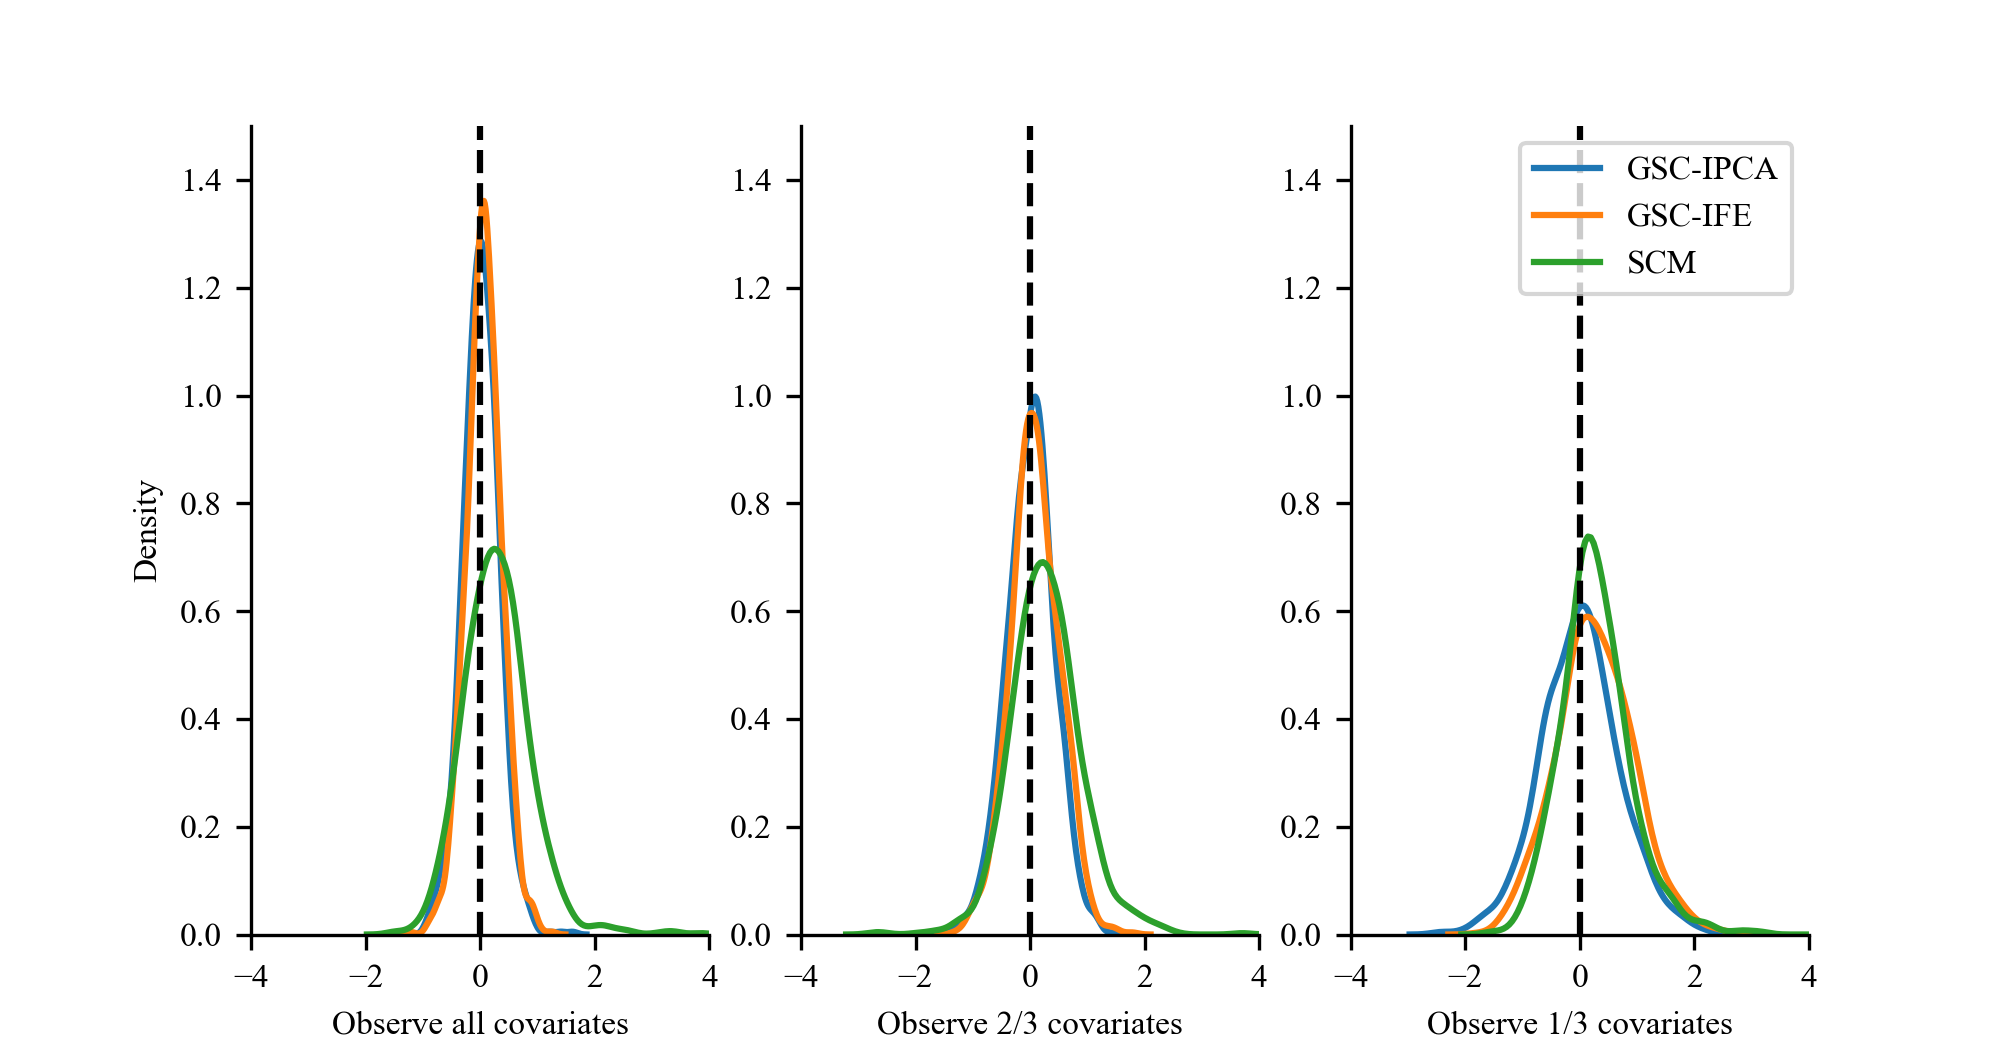
\includegraphics{figs/bias_compar2.png}
    \label{app: bias 2}
    \caption*{\footnotesize{This figure plots the CSC-IPCA, CSC-IFE, and SCM method estimated ATT for simulated data with different data generating processes.}}
    \end{figure}

\subsection{Finite sample properties}
\label{app: finite sample}
In this section, we provide additional simulation results to investigate the finite sample properties of the CSC-IFE and SCM methods for comparision.

\begin{table}[!ht]
    \centering
    \caption{\textbf{Finite Sample Properties of CSC-IFE}}
    \begin{tabular}{cc|ccc|ccc|ccc}
    \toprule
    \multicolumn{2}{c|}{$\alpha$} & $1/3$ & $2/3$ & 1 & $1/3$ & $2/3$ & 1 & $1/3$ & $2/3$ & 1 \\
    \hline
    $T_0$ & $N_{ctrl}$ & \multicolumn{3}{c|}{Bias} & \multicolumn{3}{c|}{RMSE}  & \multicolumn{3}{c}{STD} \\
    \hline
    10 & 10 & 6.478 & 3.184 & 0.045 & 7.996 & 4.311 & 0.747 & 4.701 & 2.939 & 0.854 \\
    10 & 20 & 6.173 & 2.885 & -0.018 & 8.070 & 4.050 & 0.599 & 5.245 & 2.900 & 0.769 \\
    10 & 40 & 4.510 & 2.516 & -0.007 & 6.785 & 3.931 & 0.527 & 5.096 & 3.044 & 0.675 \\
\cline{1-11}
    20 & 10 & 6.650 & 3.536 & -0.007 & 8.051 & 4.843 & 0.777 & 4.593 & 3.336 & 0.904 \\
    20 & 20 & 6.402 & 3.198 & -0.013 & 8.085 & 4.529 & 0.587 & 4.939 & 3.272 & 0.740 \\
    20 & 40 & 5.690 & 2.555 & 0.001 & 7.633 & 3.864 & 0.570 & 5.111 & 2.935 & 0.720 \\
\cline{1-11}
    40 & 10 & 7.353 & 3.523 & -0.008 & 11.132 & 5.258 & 0.696 & 8.364 & 3.950 & 0.846 \\
    40 & 20 & 6.904 & 3.230 & 0.036 & 9.185 & 5.084 & 0.602 & 6.053 & 3.935 & 0.747 \\
    40 & 40 & 5.978 & 2.928 & 0.003 & 9.368 & 4.850 & 0.650 & 7.227 & 3.927 & 0.782 \\
    \bottomrule
    \end{tabular}
    \begin{tablenotes}
        \item This table presents the finite sample properties of the CSC-IFE method estimated ATT for simulated data. The number of treated units and post-treatment period are fixed to $N_{treat} = 5, T_1=5$. We vary the number of control units $N_{ctrl}$, pre-treatment period $T_0$, and proportion of observed covariates $\alpha$ to investigate the finite sample properties, the total number of covariates is $L=9$. The bias, RMSE, and STD are estimated based on 1000 simulations.
    \end{tablenotes}
    \end{table}

\begin{table}[!ht]
    \centering
    \caption{\textbf{Finite Sample Properties of SCM}}
    \begin{tabular}{cc|ccc|ccc|ccc}
    \toprule
    \multicolumn{2}{c|}{$\alpha$} & $1/3$ & $2/3$ & 1 & $1/3$ & $2/3$ & 1 & $1/3$ & $2/3$ & 1 \\
    \hline
    $T_0$ & $N_{ctrl}$ & \multicolumn{3}{c|}{Bias} & \multicolumn{3}{c|}{RMSE}  & \multicolumn{3}{c}{STD} \\
    \hline
    10 & 10 & 10.026 & 10.188 & 9.909 & 10.997 & 11.323 & 10.964 & 4.554 & 4.960 & 4.721 \\
    10 & 20 & 9.874 & 10.007 & 9.924 & 11.011 & 11.168 & 11.028 & 4.872 & 4.991 & 4.840 \\
    10 & 40 & 9.720 & 10.088 & 9.521 & 10.891 & 11.388 & 10.655 & 4.936 & 5.304 & 4.808 \\
\cline{1-11}
    20 & 10 & 10.596 & 10.526 & 10.674 & 12.036 & 11.841 & 12.149 & 5.714 & 5.454 & 5.816 \\
    20 & 20 & 10.269 & 10.250 & 10.113 & 11.935 & 11.671 & 11.745 & 6.109 & 5.614 & 5.985 \\
    20 & 40 & 9.719 & 9.654 & 10.206 & 11.309 & 11.206 & 12.353 & 5.810 & 5.699 & 6.986 \\
\cline{1-11}
    40 & 10 & 10.678 & 11.069 & 11.117 & 12.794 & 12.946 & 13.705 & 7.087 & 6.731 & 8.033 \\
    40 & 20 & 10.970 & 11.207 & 11.148 & 13.719 & 13.459 & 13.601 & 8.249 & 7.451 & 7.780 \\
    40 & 40 & 10.742 & 10.851 & 10.221 & 13.303 & 13.786 & 12.684 & 7.853 & 8.520 & 7.539 \\
    \bottomrule
    \end{tabular}
    \begin{tablenotes}
        \item This table presents the finite sample properties of the SCM method estimated ATT for simulated data. The number of treated units and post-treatment period are fixed to $N_{treat} = 5, T_1=5$. We vary the number of control units $N_{ctrl}$, pre-treatment period $T_0$, and proportion of observed covariates $\alpha$ to investigate the finite sample properties, the total number of covariates is $L=9$. The bias, RMSE, and STD are estimated based on 1000 simulations.
    \end{tablenotes}
    \end{table}
    
\end{document}
